\documentclass{article}

\usepackage{graphicx} % Required for inserting images
\usepackage{geometry}
\usepackage{float}
\usepackage{tabularray}
\usepackage{listings}


\begin{document}

\begin{titlepage}
    \centering
    \vspace*{1cm}

    
\includegraphics[width=0.4\textwidth]{dei_thumb.png} % Replace with your university logo

    \vspace{1.5cm}
    {\LARGE \textbf{TPC-H e Benchmarking SGDs} \par}
   
    {\Large PostgreSQL vs MySQL \par}

    \vspace{2.5cm}
    \textbf{Mestrado em Engenharia Informática} \\
    \textbf{Sistemas de Gestão de Dados 2023/2024} \\
    \vspace{0.5cm} 
    \textbf{Document version: 1.0} \\
    \vspace{3cm}
    \begin{tabular}{ll}
        \textbf{Bruno Sequeira} & 2020235721, brunosequeira@student.dei.uc.pt \\
        \textbf{Rui Santos} & 2020225542, rpsantos@student.dei.uc.pt
        
      
    \end{tabular}\\
    \vspace{1.5cm} 
    \textbf{Universidade de Coimbra}

    \date{}

    \vfill

\end{titlepage}
   \clearpage
   \tableofcontents
   \clearpage
   \listoffigures
   \listoftables

\clearpage
\section{Introdução}
\quad No mundo contemporâneo, onde os dados se tornaram um ativo extremamente valioso e omnipresente em quase todos os setores da sociedade, a capacidade de gerir grandes quantidades de dados de forma eficiente tornou-se uma prioridade fundamental. Empresas, organizações governamentais, instituições académicas e até mesmo indivíduos enfrentam o desafio de lidar com volumes massivos de dados, muitas vezes provenientes de diversas fontes e em formatos diversos.\\

\quad Nesse contexto, os sistemas de gestão de dados (SGDs) desempenham um papel crucial. Essas ferramentas oferecem estruturas e mecanismos para armazenar, organizar, recuperar e manipular dados de maneira eficaz. No entanto, à medida que a quantidade e a complexidade dos dados aumentam, os desafios enfrentados pelos SGBDs também crescem exponencialmente.\\

\quad O objetivo deste projeto é explorar e entender como os motores de base de dados tradicionais lidam com grandes volumes de dados e consultas complexas de forma eficiente. Para alcançar esse objetivo, iremos utilizar o TPC-H como benchmarking. O TPC-H é um conjunto padrão de consultas de benchmarking projetado para avaliar o desempenho de SGBDs em cenários de análise de dados complexos.\\

\quad Este projeto se concentrará em dois dos SGDs mais amplamente utilizados e estabelecidos no mercado: MySQL e PostgreSQL. Ambos são sistemas de código aberto com uma vasta base de utilizadores e uma longa história de desenvolvimento. Ao comparar o desempenho desses dois SGBDs em relação ao benchmark TPC-H, pretendemos obter insights valiosos sobre suas capacidades e limitações no processamento de grandes quantidades de dados e consultas complexas.\\

\quad Ao finalizar este projeto, esperamos não apenas aumentar nossa compreensão sobre como os motores de base de dados tradicionais lidam com grandes volumes de dados e consultas complexas, mas também fornecer insights práticos e acionáveis para otimizar o desempenho e a eficiência do gestão de dados em ambientes do mundo real.\\
\clearpage

\section{Estrutura da Base de Dados}
Apresentamos agora a estrutura da nossa base de dados, terá cerca de 8 tabelas.\\

As tabelas são: lineitem, partsupp, part, supplier, nation, region, orders e customer. Sendo que estas têm ligações umas às outras.
\begin{figure}[H]
  \centering
  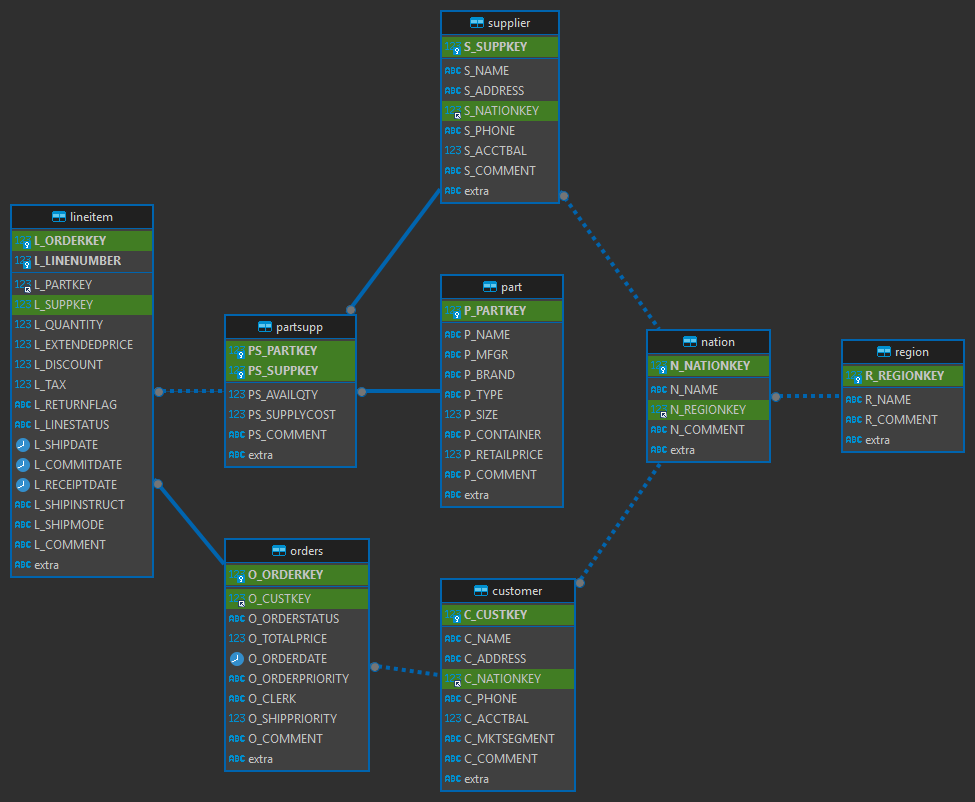
\includegraphics[width=\textwidth]{Graphs/tpchassignment.png}\\
  \caption{Imagem - Estrutura da base de dados.}
  \label{fig:row_import_time}
\end{figure}

\clearpage


\section{Especificações e Configurações do Computador}

\quad Nesta seção, vamos nos aprofundar nas especificações e configurações do hardware do computador que utilizamos para realizar nossos testes de desempenho e análises comparativas entre diferentes sistemas de gestão de base de dados (SGBDs). A escolha adequada do hardware é fundamental para garantir resultados precisos e significativos nas nossas experiências.\\

(AGORA CONTIGO RUI) (FAZER Benchmarking com o ssd, configurações)


\section{Criação de Dados}

\quad Para realizar nossos testes de desempenho e análises comparativas entre diferentes SGBDs, como PostgreSQL e MySQL, decidimos gerar um conjunto de dados TPC-H usando o dbgen. Este conjunto de dados terá aproximadamente 25GB de tamanho, proporcionando uma carga de trabalho significativa para os sistemas em teste.\\

\quad O dbgen é uma ferramenta versátil que nos permite configurar diversos parâmetros, como o fator de escala, para ajustar o tamanho do conjunto de dados gerado de acordo com nossos requisitos específicos. Além disso, ele produz dados realistas e consistentes, conforme definido pelas especificações do TPC-H.


\quad Após instalação dessa feramenta, utilizamos o seguinte comando \textbf{dbgen -s 25}.

\quad O dbgen gerará 8 arquivos .tbl (dados de tabela).




\section{Plano de Execução}


\quad Para cada motor (mysql e postgres) iremos seguir o seguinte plano:

\begin{enumerate}
    \item Tempos de Importação dos dados, sem as chaves(PK's e FK's).
    \item Tempos de Execução de cada query, sem as chaves(PK's e FK's).
    \item Tempos de Importação de criação de cada chave PK e FK.
    \item Tempos de Execução da pesquisa de cada query, com as chaves (PK's e FK's).
    \item Explain plan de uma query rápida e de uma lenta.
    \item Explain plan mysql vs postgres para uma query lenta.
\end{enumerate}

\quad Os quatro primeiros passos esses tempos irão ser executados 5 vezes, sendo no final apresentado o valor de todos, a cold run finalizando com a média total.\\

\section{Scripts e código utilizado}
\quad Inicialmente criamos vários scripts, dos quais foram todos submetidos na entrega. Iremos agora explicar a função de cada script.\\

\quad Estes scripts estão divididos por cada motor de pesquisa, mas contêm o mesmo nome.\\

\begin{itemize}
    \item \textbf{CreateDB.sh} este script irá criar uma nova base de dados, com nome "tpch-cloud".
    \item \textbf{CreateTables.sh} irá criar todas as 8 tabelas do tpc-h (customer, lineitem, nation, orders, part, partsupp, region e supplier).
    \item \textbf{ImportData.sh} irá importar os dados anteriormente gerados pelo database generator para a base de dados "tpch-cloud", colocando o resultado do tempo de execução de cada tabela no ficheiro Results/ImportTime.txt
    \item \textbf{DropColumnExtra.sh} irá eliminar de todas as tabelas a ultima coluna, isto porque foi necessário criar uma nova columa por tabela para que a importação fosse concluída com sucesso.
    \item \textbf{CreatePK.sh} criação das chaves primárias (PK's), colocando o tempo de criação no ficheiro Results/PKCreation.txt
    \item \textbf{CreateFK.sh} criação das chaves estrangeiras (FK's), colocando os resultados no ficheiro Results/FKCreation.txt
    \item \textbf{Search.py} este código em python usa multithreading para executar consultas SQL na base de dados PostgreSQL/MySQL. Ele cria várias threads(1 a 5) que executam consultas SQL em paralelo, controlando o acesso a uma lista compartilhada de consultas e registrando os resultados em um arquivo de texto. O tempo de execução de cada query é colocado num ficheiro com nome Results/ExecutionTime.txt .
     
\end{itemize}

\clearpage

\section{Resultados - Tabelas}

\subsection{Importação dos Dados}
\quad Após criação dos dados pelo dbgen referidos anteriormente, criando cerca de 25GB de dados, iremos prosseguir com a importação desses dados para a base de dados. \\
Para isso, foi utilizado o script \textbf{\textit{ImportData.sh}}, que irá guardar o tempo de importação de cada tabela num ficheiro. \\
\quad Apresentamos agora uma tabela que contém a média dos tempos de importação para cada tabela, por cada motor de pesquisa MySQL e PostgreSQL, e outras informações que são importantes para análise, o tamanho do ficheiro de cada tabela, e o número de linhas que cada tabela apresenta.
\quad Na próxima secção iremos fazer uma análise mais extensiva com estes dados.\\
\begin{table}[H]
    \centering
    \renewcommand{\arraystretch}{1.7}
    \resizebox{\textwidth}{!}{%
    \begin{tabular}{|l|r|r|r|r|}
        \hline  
        \textbf{Table} & \textbf{MySQL (s)} & \textbf{PostgreSQL (s)} & \textbf{Size (KB)} & \textbf{Rows} \\ \hline
        region.tbl & 0,016 & 0,0076 & 1 & 5 \\ \hline
        nation.tbl & 0,000 & 0,0060 & 3 & 25 \\ \hline
        supplier.tbl & 4,609 & 0,733 & 28 000 & 200 000  \\ \hline
        part.tbl & 62,11 & 12,919 & 481 682 & 4 000 000 \\ \hline
        customer.tbl & 54,391 & 10,794 & 482 234 & 3 000 000  \\ \hline
        partsupp.tbl & 260,234 & 50,526 & 2 381 754 & 16 000 000 \\ \hline
        orders.tbl & 594,343 & 120 & 3 464 345 & 30 000 000 \\ \hline
        lineitem.tbl & 2861,766 & 754 & 15 434 957 & 119 994 608 \\ \hline
    \end{tabular}}
    \caption{Tempo de importação com 25GB de base de dados. Informações acerca de cada tabela.}
    \label{tab:BC_Table1}
  \end{table}


\clearpage
\subsection{Criação das chaves primárias e estrangeiras(PK e FK)}

\quad Após importação dos dados, iremos criar as chaves primárias e estrangeiras, utilizando os scripts \textbf{\textit{CreatePK.sh}},\textbf{\textit{CreateFK.sh}}, respetivamente.\\
\quad As próximas tabelas apresentam as médias dos tempos de criação de cada chave por cada motor de pesquisa MySQL e PostgreSQL.\\

\begin{table}[H]
    \centering
    \renewcommand{\arraystretch}{1.7}
    \resizebox{\textwidth}{!}{%
    \begin{tabular}{|l|r|r|}
        \hline  
        \textbf{Table} & \textbf{MySQL (s)} & \textbf{PostgreSQL (s)} \\ \hline
        R\_REGIONKEY into Table REGION & 0.07472675 & 0,104\\ \hline
        N\_NATIONKEY into Table NATION & 0,06011025 & 0.06  \\ \hline
        C\_CUSTOMERKEY into Table CUSTOMER & 20,0989515 & 2,649  \\ \hline
        S\_SUPPKEY into Table SUPPLIER & 2,43648875 & 0,307 \\ \hline
        P\_PARTKEY into Table PART & 29,07967075 & 3,581  \\ \hline
        PS\_PARTKEY,PS\_SUPPKEY into Table PARTSUPP & 145,130026 & 11,583 \\ \hline
        O\_ORDERKEY into Table ORDERS & 225,7778648 & 20,725 \\ \hline
        L\_ORDERKEY,L\_LINENUMBER into Table LINEITEM & 1135,13439 & 96 \\ \hline
    \end{tabular}}
    \caption{Tempo de criação das chaves primárias em segundos para cada motor de pesquisa.(PK)}
    \label{tab:BC_Table2}
  \end{table}




\begin{table}[H]
    \centering
    \renewcommand{\arraystretch}{1.7}
    \resizebox{\textwidth}{!}{%
    \begin{tabular}{|l|r|r|}
        \hline  
        \textbf{Name} & \textbf{MySQL (s)} & \textbf{PostgreSQL (s)}\\ \hline
    
        SUPPLIER ADD FOREIGN KEY (S\_NATIONKEY) &	3,451038 &	0,157 \\ \hline
        NATION ADD FOREIGN KEY (N\_REGIONKEY) & 	0,08686725   &	0,061 \\ \hline
        CUSTOMER ADD FOREIGN KEY (C\_NATIONKEY) &  48,40295275 &	1,658 \\ \hline
        PARTSUPP ADD FOREIGN KEY (PS\_SUPPKEY) &	971,6817368	& 6,108 \\ \hline
        PARTSUPP ADD FOREIGN KEY (PS\_PARTKEY) & 1008,497317	& 2,491 \\ \hline
        ORDERS ADD FOREIGN KEY (O\_CUSTKEY) & 8743,760717	& 23,338 \\ \hline 
        LINEITEM ADD FOREIGN KEY (L\_ORDERKEY) &	2180,671 & 35,203 \\ \hline
        LINEITEM ADD FOREIGN KEY (L\_PARTKEY, L\_SUPPKEY)   REFERENCES PARTSUPP & 12967,219 &	131 \\ \hline
 \end{tabular}}
    \caption{Tempo de criação das chaves estrangeiras em segundos para cada motor de pesquisa.(FK)}
    \label{tab:BC_Table3}
  \end{table}
\clearpage


\subsection{Tempo de execução sem PK's e FK's utilizando 1 thread numa base de dados de 25GB.}
\quad A próxima tabela apresenta os tempos de pesquisa de cada query para o motor de pesquisa PostgreSQL, utilizando uma thread e sem chaves, para isso foi utilizado o ficheiro Python \textbf{\textit{Search.py}}  com a variável \textit{num\_threads} a 1. 
\quad É apresentado a Cold Run que se refere à primeira execução de cada query quando o sistema está num estado onde os dados não estão em cache.\\
Foram executadas mais 5 vezes para que os dados finais fossem mais consistentes.\\
NOTA: A query 2, 17 e 20, os resultados estão a 0, mas na realidade estes demoraram mais que 1h para executar, mas não deixamos a pesquisa ir até ao fim.

  \begin{table}[H]
    \centering
    \renewcommand{\arraystretch}{1.4}
    \resizebox{\textwidth}{!}{% \textbf{\textit{Search.py}} 
    \begin{tabular}{|l|r|r|r|r|r|r|}
        \hline  
        \textbf{Query} & \textbf{1st} & \textbf{2nd} & \textbf{3rd} &\textbf{4th} &\textbf{5th} & \textbf{Cold-Run} \\ \hline
        Q1	&116,8099941&	120,0591266&	117,8674161	&114,4022444&	115,6990086&	122,7438045 \\ \hline
        Q2&	0&	0	&0&	0&	0	&0 \\ \hline
        Q3&	53,41674374	&54,93958569&	53,00420475	&49,26812755&	52,34300213	&51,83544731 \\ \hline
        Q4&	103,2836877	&109,0401967&	100,2488358	&98,64638119&	102,5063354	&101,3624349 \\ \hline
        Q5&	71,68611916	&74,19141603&	74,53215671	&72,45572729&	75,21843824	&69,95115733 \\ \hline
        Q6&	34,57011132	&34,93635273&	34,44202471	&30,41916679&	35,19708422	&33,7043817 \\ \hline
        Q7&	46,93297661	&45,13665271&	45,10902643	&46,2673193	&45,39536603	&45,00285292 \\ \hline
        Q8&	81,31571231	&82,22141171	&81,50476956	&77,59742372&	82,13007905	&80,97627687 \\ \hline
        Q9&	153,1270361	&167,0394394	&152,053899&	148,13301	&150,7011644	&145,0627949 \\ \hline
        Q10	&56,066711	&56,13991499	&56,08217931&	54,88764372	&57,20420032	&52,98872352 \\ \hline
        Q11	&6,787621341	&6,34415555	&6,475395918&	8,188070274	&3,694438541	&6,214289427 \\ \hline
        Q12&	47,9200356	&46,89917636&	49,35352349	&45,76049022&	47,66896127	&47,71614718 \\ \hline
        Q13&	25,15876964	&22,04244781&	24,45808411	&24,36592422&	24,24460123	&22,57851076 \\ \hline
        Q14&	37,80597485	&38,27917409&	36,8521173	&36,16681273&	36,20820179	&35,94376898 \\ \hline
        Q15&	71,08209229	&71,43925333&	72,44926357	&73,4770297&	72,39981597&	71,26171803 \\ \hline
        Q16&	11,12500028&	10,81070876&	12,39403391	&11,27183321	&13,11927584&	12,02717423 \\ \hline
        Q17&	0&	0	&0&	0&	0	&0 \\ \hline
        Q18&	514,0775939	&516,8559051	&511,7627821&	515,4603785	&518,0354649&	526,8242321 \\ \hline
        Q19&	34,9657512	&35,70931292&	37,91975284	&38,59785392	&37,46897349&	36,41795897 \\ \hline
        Q20&	0&	0	&0&	0	&0&	0 \\ \hline
        Q21	&0&	0	&0&	0&	0	&0 \\ \hline
        Q22&	13,4014403	&12,87695646	&12,88543606	&12,38910711	&13,10658183&	12,59100842 \\ \hline
      \end{tabular}}
      
    \caption{Tempo de pesquisa de cada query no PostgresSQL.(1 Thread)}
    \label{tab:BC_Table3}
  \end{table}
\clearpage

\quad A próxima tabela apresenta os tempos de pesquisa de cada query para o motor de pesquisa MySQL, utilizando uma thread sem chaves, para isso foi utilizado o ficheiro Python \textbf{\textit{Search.py}}  com a variável \textit{num\_threads} a 1. 
\quad É apresentado a Cold Run que se refere à primeira execução de cada query quando o sistema está num estado onde os dados não estão em cache.\\
Foram executadas mais 5 vezes para que os dados finais fossem mais consistentes.\\
NOTA: A query 2,17,19,30 e 21 os resultados estão a 0, mas na realidade estes demoraram mais que 1h para executar, mas não deixamos a pesquisa ir até ao fim.


  \begin{table}[H]
    \centering
    \renewcommand{\arraystretch}{1.4}
    \resizebox{\textwidth}{!}{%
    \begin{tabular}{|l|r|r|r|r|r|r|}
        \hline  
        \textbf{Query} & \textbf{1st} & \textbf{2nd} & \textbf{3rd} &\textbf{4th} &\textbf{5th} & \textbf{Cold-Run} \\ \hline
     
Q1	&432,3271651	&431,8597636	&431,829649&	436,1161312	&430,097073&	508,8306904 \\ \hline
Q2	&0&	0&	0&	0&	0&	0\\ \hline
Q3	&263,3187106	&297,865124	&274,9916154&	260,9870513	&265,5107948&	313,7286842\\ \hline
Q4	&332,4258604&	391,1751814	&330,5995704&	322,7159381	&333,8759478	&375,8153143\\ \hline
Q5	&1778,683372&	2042,87998	&1789,041688&	1782,216714&	1784,398126	&1964,174181\\ \hline
Q6	&152,5687261&	182,7490625	&146,7618471&	160,8769024&	144,1799477&	174,5804477\\ \hline
Q7	&2211,592215&	2469,019428	&2214,303127&	2203,169617&	2205,734095&	2604,254816\\ \hline
Q8	&1854,861638&	2307,910877	&1859,425241&	1853,458512	&1848,857935	&2200,514827\\ \hline
Q9	&1340,716846&	1820,645067	&1338,06962	&1344,136749&	1338,362	&1621,757987\\ \hline
Q10	&434,8548419&	431,0802007	&443,4370315&	432,444042&	430,086104&	405,8647189\\ \hline
Q11	&52,5315187	&55,27335548	&60,28759084&	58,89543221&	51,87436561&	48,1277492\\ \hline
Q12	&222,2177103&	267,7758906	&213,8883981&	211,0139893	&222,5429354&	204,2217941\\ \hline
Q13	&275,9721282&	409,3423953	&275,822865	&272,3186603&	279,1985606	&258,0313485\\ \hline
Q14	&158,3711605&	180,5114081	&158,1940707&	161,2790932	&164,3283402	&161,4675171\\ \hline
Q15	&0,014033794&	0,038739204	&8,656888316&	2,572689486&	1,246914389	&0,055614233\\ \hline
Q16	&39,77274013&	42,2590394	&31,93049952&	33,59717521	&34,51469057	&36,18514109\\ \hline
Q17	&0	&0	&0	&0	&0	&0\\ \hline
Q18	&1997,829578	&1852,838384&	2007,350438	&1994,420447&	2001,535017	&1689,722517\\ \hline
Q19	&0	&0	&0	&0	&0	&0\\ \hline
Q20	&0	&0	&0	&0	&0	&0\\ \hline
Q21	&0	&0	&0	&0	&0	&0\\ \hline
Q22	&187,2806194&	138,7884924&	179,4008842	&180,2004963	&188,1653592&	138,4675019\\ \hline    \end{tabular}}
    \caption{Tempo de pesquisa de cada query no MySQL.(1 Thread, sem chaves)}
    \label{tab:BC_Table3}
  \end{table}





\clearpage
\subsection{Tempo de execução sem PK's e FK's utilizando 5 thread numa base de dados de 25GB.}
\quad A próxima tabela apresenta os tempos de pesquisa de cada query para o motor de pesquisa PostgreSQL, utilizando 5 thread's e sem chaves, para isso foi utilizado o ficheiro Python \textbf{\textit{Search.py}}  com a variável \textit{num\_threads} a 5. 
\quad É apresentado a Cold Run que se refere à primeira execução de cada query quando o sistema está num estado onde os dados não estão em cache.\\
Foram executadas mais 5 vezes para que os dados finais fossem mais consistentes.\\
NOTA: A query 2, 17 e 20, os resultados estão a 0, mas na realidade estes demoraram mais que 1h para executar, mas não deixamos a pesquisa ir até ao fim.

  \begin{table}[H]
    \centering
    \renewcommand{\arraystretch}{1.4}
    \resizebox{\textwidth}{!}{% \textbf{\textit{Search.py}} 
    \begin{tabular}{|l|r|r|r|r|r|r|}
        \hline  
        \textbf{Query} & \textbf{1st} & \textbf{2nd} & \textbf{3rd} &\textbf{4th} &\textbf{5th} & \textbf{Cold-Run} \\ \hline
        Q1	&237,7450857&	261,1408794&	267,2472773	&262,5045719&	264,2472773&	271,6175628 \\ \hline
        Q2	&0	&0&	0	&0	&0	&0  \\ \hline
        Q3	&318,5259473&	148,5627244&	142,5581777&	144,8695186	&144,5581777&	138,6535156 \\ \hline
        Q4	&230,6480374	&241,7291894&	246,7411501&	250,4226668	&245,7411501	&251,7409484 \\ \hline
        Q5	&226,354182	&415,4596763&	381,7220685	&378,1967514	&377,7220685	&384,9668825 \\ \hline
        Q6	&87,8208189	&115,3777912&	113,2136195	&112,2827849	&117,2136195	&105,0868742 \\ \hline
        Q7	&113,1751678	&172,6041148&	157,7151744&	161,1033752	&154,7151744	&161,4731843 \\ \hline
        Q8&	176,6483243	&180,6843915	&176,2252629	&176,7249143	&171,2252629	&171,4162769 \\ \hline
        Q9	&301,855588	&294,7246604	&275,7119792	&279,3611783	&277,7119792	&279,0646768 \\ \hline
        Q10	&190,3323045	&146,1063757	&133,1834276	&135,5568994&	128,1834276	&183,629493 \\ \hline
        Q11	&51,66847563	&39,64738894	&33,70240498	&30,77221727&	38,70240498	&29,84241724 \\ \hline
        Q12	&122,5441322	&136,2984984	&143,5715346	&141,4268394&	147,5715346	&111,3740797 \\ \hline
        Q13	&111,324209	&52,8677969&	48,44592786&	51,70726744&	52,44592786	&49,63776112 \\ \hline
        Q14&	89,50986934	&83,71655297	&86,9114275	&89,46507604&	81,9114275	&84,06736493 \\ \hline
        Q15&	143,9871836&	138,3716445	&196,948508	&192,7949816&	198,948508	&215,9613121 \\ \hline
        Q16&	35,39535165&	47,01218653&	22,71657276&	27,30784579	&21,71657276	&24,29615664 \\ \hline
        Q17	&0&	0	&0	&0	&0	&0 \\ \hline
        Q18	&714,5049183	&653,9689264	&556,1102753&	549,3142951&	551,1102753	&548,5621278 \\ \hline
        Q19	&91,73884964	&81,06190705	&96,1268611&	95,87672346&	91,1268611	&80,66898918 \\ \hline
        Q20	&0	&0&	0	&0&	0&	0 \\ \hline
        Q21&	0	&0&	0	&0&	0&	0 \\ \hline
        Q22	&47,10031652&	39,94770336	&45,13888717	&44,68222742&	44,13888717	&42,95714927 \\ \hline   \end{tabular}}
      
    \caption{Tempo de pesquisa de cada query no PostgresSQL.(5 Thread's, sem chaves)}
    \label{tab:BC_Table3}
  \end{table}
\clearpage

\quad A próxima tabela apresenta os tempos de pesquisa de cada query para o motor de pesquisa MySQL, utilizando 5 thread's e sem chaves, para isso foi utilizado o ficheiro Python \textbf{\textit{Search.py}}  com a variável \textit{num\_threads} a 5. 
\quad É apresentado a Cold Run que se refere à primeira execução de cada query quando o sistema está num estado onde os dados não estão em cache.\\
Foram executadas mais 5 vezes para que os dados finais fossem mais consistentes.\\
NOTA: A query 2,17,19,30 e 21 os resultados estão a 0, mas na realidade estes demoraram mais que 1h para executar, mas não deixamos a pesquisa ir até ao fim.


  \begin{table}[H]
    \centering
    \renewcommand{\arraystretch}{1.4}
    \resizebox{\textwidth}{!}{%
    \begin{tabular}{|l|r|r|r|r|r|r|}
        \hline  
        \textbf{Query} & \textbf{1st} & \textbf{2nd} & \textbf{3rd} &\textbf{4th} &\textbf{5th} & \textbf{Cold-Run} \\ \hline
     
        Q1&	508,9230449	&508,9230449	&453,8894722	&456,5680265	&450,9159719	&840,164 \\ \hline
        Q2&	0&	0	&0	&0&	0&	0 \\ \hline
        Q3&	346,389854&	336,0984678&	284,5237944	&302,7604377	&295,0102452&	499,8198061 \\ \hline
        Q4&	417,8754093	&424,3258688	&366,5896633&	380,9676487&	371,826259	&671,0322769 \\ \hline
        Q5&	844,6286964	&844,6286964	&787,422472	&1358,901059	&821,1231287&	1326,647805 \\ \hline
        Q6&	201,2151916	&201,2151916	&175,5249379&	179,4729862&	172,8457361&	285,9920955 \\ \hline
        Q7&	2758,015287	&2768,318821	&1109,288278&	859,4860127&	856,7565462&	3522,377851 \\ \hline
        Q8&	1440,221793	&1446,924434	&2579,901866&	1055,858156	&1050,66304	&826,5577955 \\ \hline
        Q9&	878,4390702	&878,4390702	&1333,149814&	388,7902443	&395,52546&	655,5954437 \\ \hline
        Q10&	1183,287196&	1172,826146	&1358,690806&	1111,425853	&1119,14447&	884,0797031 \\ \hline
        Q11	&72,06504185&	62,51723695&	64,37585354	&65,40043664&	58,38949597	&92,09835458 \\ \hline
        Q12	&272,0332285&	262,895956	&242,7265551	&250,5499992&	258,1605387&	343,5871196 \\ \hline
        Q13	&710,4044674&	702,4743304	&772,9322371	&477,6072123&	481,9663019	&479,8104253 \\ \hline
        Q14	&188,5136945&	180,8245311	&182,9520864	&180,4727402&	171,8743046	&247,8809063 \\ \hline
        Q15	&9,768925217&	0,128311157	&0,273048639	&0,012115955&	4,27E-03&	0,047004938 \\ \hline
        Q16	&45,55357562&	45,86201859	&64,52356267	&57,37397313&	50,13349683	&63,13711166 \\ \hline
        Q17	&0&	0	&0	&0&	0&	0 \\ \hline
        Q18	&1779,232895	&1779,232895&	1764,878921&	1787,270872	&1779,360765&	2113,106026 \\ \hline
        Q19	&0&	0	&0	&0&	0&	0 \\ \hline
        Q20	&0&	0	&0	&0&	0&	0 \\ \hline
        Q21	&0&	0	&0	&0&	0&	0 \\ \hline
        Q22	&143,3749725&	153,2982109	&150,3335512	&145,6784673&	138,4015162&	202,4831903 \\ \hline \end{tabular}}
    \caption{Tempo de pesquisa de cada query no MySQL.(5 Thread's, sem chaves)}
    \label{tab:BC_Table3}
  \end{table}


\clearpage
\subsection{Médias e Desvio padrão de tempos entre MySQL vs PostgresSQL, sem chaves utilizando 1 thread's.}

  \quad Para uma melhor comparação entre os dois motores de pesquisa, iremos apresentar uma tabela com a médias e desvios padrão de cada query para o MySQL e PostgreSQL, sem chaves utilizando 1 thread. \\
NOTA: Nas querys 2,17,20,21 não é possível ter uma análise, visto que não foi concluída nem no PostgreSQL nem o MySQL. A query 19 não foi concluída no MySQL, portanto podemos concluir que no PostgreSQL foi mais rápido. O valor de 0 significa que demorou imenso tempo perto de 1 hora.

  \begin{table}[H]
    \centering
    \renewcommand{\arraystretch}{1.4}
    \resizebox{\textwidth}{!}{%
    \begin{tabular}{|l|r|r|r|r|}
        \hline 
    
        \textbf{Query} & \textbf{Média PostgreSQL} & \textbf{Média MySQL} & \textbf{Desvio PostgreSQL} &\textbf{Desvio MySQL} \\ \hline
        Q1 &	116,967558	&432,4459564 & 1,927818415& 1,986202646\\ \hline
        Q2	&0&	0& 0 &0\\ \hline
        Q3	&52,59433277&	272,534659 &1,86929796   &13,52985373\\ \hline
        Q4	&102,7450874&	342,1584996& 3,549821348 &24,80960324\\ \hline
        Q5	&73,61677148&	1835,443976& 1,327322483 &103,7723032\\ \hline
        Q6&	33,91294795	& 157,4272972& 1,767181713 &13,89921858\\ \hline
        Q7&	45,76826821	&2260,763697 &0,718079597 &104,2038425\\ \hline
        Q8&	55,8536493	&1944,902841 &1,714075934 &181,53532\\ \hline
        Q9&	80,95387927	&1436,386056& 6,628089139 &192,1418003\\ \hline
        Q10&	154,2109098&	434,380444&0,733380679 &4,802696029\\ \hline
        Q11&	56,07612987	&55,77245257& 1,457684918 &3,349247904\\ \hline
        Q12&	47,52043739	&227,4877847& 1,185354128& 20,64793427\\ \hline
        Q13&	24,0539654	&302,5309219 &1,054871338 &53,45008983\\ \hline
        Q14&	37,06245615	&164,5368145 &0,849634354  &8,29565594\\ \hline
        Q15&	72,16949097	&2,505853038& 0,84340533 &3,216222705\\ \hline
        Q16&	11,7441704	&36,41482897 &0,870753953 &3,926557581\\ \hline
        Q17&	0	&0& 0  &0\\ \hline
        Q18&	515,2384249&	1970,794773 &2,187078412 &59,13381791\\ \hline
        Q19&	36,93232887&	0& 1,371142809 &0\\ \hline
        Q20&	0	&0 &0  &0\\ \hline
        Q21&	0	&0 &0 &0\\ \hline
        Q22&	12,93190435	&11,56787486 &0,331898673 &18,3387866\\ \hline
    \end{tabular}}
    \caption{Média e desvio padrão do tempo de pesquisa de cada query entre MySQL e PostgreSQL.(1 thread e sem chaves)}
    \label{tab:BC_Table6}
  \end{table}

  \clearpage

  \subsection{Médias e Desvio padrão de tempos entre MySQL vs PostgresSQL, sem chaves utilizando 5 thread's.}

  \quad Para uma melhor análise entre os dois motores de pesquisa, iremos apresentar uma tabela com a médias e desvios padrão de cada query para o MySQL e PostgreSQL, sem chaves utilizando 5 threads. \\
NOTA: Nas querys 2,17,20,21 não é possível ter uma análise, visto que não foi concluída nem no PostgreSQL nem o MySQL. A query 19 não foi concluída no MySQL, portanto podemos concluir que no PostgreSQL foi mais rápido. O valor de 0 significa que demorou imenso tempo perto de 1 hora.

  \begin{table}[H]
    \centering
    \renewcommand{\arraystretch}{1.4}
    \resizebox{\textwidth}{!}{%
    \begin{tabular}{|l|r|r|r|r|}
        \hline 
        
        \textbf{Query} & \textbf{Média PostgreSQL} & \textbf{Média MySQL} & \textbf{Desvio PostgreSQL} &\textbf{Desvio MySQL} \\ \hline
        Q1&258,5770183 &	475,8439121	&10,61408218 &27,06812684\\ \hline
        Q2&0	&	0& 0 &0\\ \hline
        Q3&	179,8149092&312,9565598&	69,38260969&24,03242114\\ \hline
        Q4&243,0564388	&392,3169698&	6,793763351& 24,03486663\\ \hline
        Q5& 355,8909493		&931,3408106&	66,28665116&214,8051085\\ \hline
        Q6&109,1817268	&186,0548087	& 10,81724197&12,55669213\\ \hline
        Q7&	151,8626013&1670,372989	&	20,27170234 &896,9700415\\ \hline
        Q8&176,3016312	&1514,713858	&3,009428515 &560,4750992\\ \hline
        Q9&285,873077	&774,8687317	&10,45033433& 353,8613607\\ \hline
        Q10&146,6724869	&1189,074894&	22,60024989&89,42786448\\ \hline
        Q11&38,89857836	&257,2732555	&7,165297481& 4,456755732\\ \hline
        Q12&	138,2825079&629,076909	&8,669249153& 10,07042702\\ \hline
        Q13&63,35822581	&24,0539654	&24,03324509 &124,3224102\\ \hline
        Q14&86,30287067	&180,9274714	&3,053802124 &5,363339509\\ \hline
        Q15&174,2101651	&2,037333955	&27,10070636& 3,867025627\\ \hline
        Q16& 30,8297059		&52,68932537	&9,423305407 &7,294633631\\ \hline
        Q17&	0	&0& 0  & 0\\ \hline
        Q18&605,0017381	&1777,99527&	67,5047972&7,252632683\\ \hline
        Q19&91,18624047	&0& 5,462991722	&0\\ \hline
        Q20&	0	&0 &0  &0\\ \hline
        Q21&	0	&0 &0 &0\\ \hline
        Q22&44,20160433	&146,2173436	&2,349963274 &5,225676328\\ \hline
    
      \end{tabular}}
    \caption{Média e desvio padrão do tempo de pesquisa de cada query entre MySQL e PostgreSQL.(5 threads sem chaves)}
    \label{tab:BC_Table6}
  \end{table}

  \clearpage

\subsection{Tempo de execução com PK's e FK's utilizando 1 thread numa base de dados de 25GB.}
\quad A próxima tabela apresenta os tempos de pesquisa de cada query para o motor de pesquisa PostgreSQL, utilizando uma thread, para isso foi utilizado o ficheiro Python \textbf{\textit{Search.py}}  com a variável \textit{num\_threads} a 1. 
\quad É apresentado a Cold Run que se refere à primeira execução de cada query quando o sistema está num estado onde os dados não estão em cache.\\
Foram executadas mais 5 vezes para que os dados finais fossem mais consistentes.\\
NOTA: A query 17 e 20, os resultados estão a 0, mas na realidade estes demoraram mais que 1h para executar, mas não deixamos a pesquisa ir até ao fim.

  \begin{table}[H]
    \centering
    \renewcommand{\arraystretch}{1.4}
    \resizebox{\textwidth}{!}{% \textbf{\textit{Search.py}} 
    \begin{tabular}{|l|r|r|r|r|r|r|}
        \hline  
        \textbf{Query} & \textbf{1st} & \textbf{2nd} & \textbf{3rd} &\textbf{4th} &\textbf{5th} & \textbf{Cold-Run} \\ \hline
        Q1 & 64,00015402&	57,86094189	&66,37642455	&66,11274171&	62,32780385	&69,58133435 \\ \hline
        Q2 & 11,28915262&	10,11524606	&11,80016232	&11,82329512&	15,18870997	&12,4443078 \\ \hline
        Q3 & 30,11691999&	28,07052135&	31,22902918	&30,85128093	&31,05623245	&30,22173095\\ \hline
        Q4	&39,68054295&	35,46339226	&36,98594427	&41,93736815	&56,70363688	&37,81141567\\ \hline
        Q5	&30,45751405&	28,15517783	&29,71593308	&36,1554563	&32,27960658&	29,58829546\\ \hline
        Q6	&22,36488271&	20,41100931	&20,44359207	&25,23021626&	24,14268041	&20,73953176\\ \hline
        Q7	&29,96915531&	27,05023456	&27,56078315	&34,33660674&	30,99301481	&28,38418627\\ \hline
        Q8	&30,42154288&	27,33011436	&27,94420171	&34,35566282&	32,66644096	&28,02946162\\ \hline
        Q9	&45,23501515&	39,44073081	&43,99806118	&56,27742958&	62,6246078	&47,01328325\\ \hline
        Q10	&31,43968391&	28,55231476	&31,51226592	&36,51843905&	33,11083174	&31,12740397\\ \hline
        Q11	&6,576447248&	6,013448715	&6,659135342&	8,271252871	&8,129918814	&6,606197119\\ \hline
        Q12	&28,57990193&	25,05599856	&28,89467883&	33,53329825&	32,53856039&	27,93996549\\ \hline
        Q13	&58,00455022&	50,90825415	&60,45565963&	72,7278986	&68,86041451&	62,51581645\\ \hline
        Q14	&19,63748908&	18,72085452	&18,73987103&	21,14933753	&23,41367555	&19,12004519\\ \hline
        Q15	&37,05613351&	35,27413845	&36,96409917&	38,18985558	&41,3369441	&35,99690318\\ \hline
        Q16	&10,07043123&	8,520478964	&9,87141633	&10,57068014	&12,55969501&	10,03213358\\ \hline
        Q17	&	0	&0&	0		&0 & 0 & 0\\ \hline
        Q18	&221,9130883	&216,5773327&	242,1048627&	230,458416	&284,6776071 &	221,2155542\\ \hline
        Q19	&19,47276449&	20,86533117	&21,04702854	&22,28647327&	22,35616946&	21,30062103\\ \hline
        Q20	&	0	&0&	0		&0 & 0 & 0\\ \hline
        Q21&	170,3248016&		168,6722145	&	173,8977368&		168,2696544	&	170,4502889	&	174,6696872\\ \hline
        Q22	&9,354454279&	11,02853131	&11,2479372&	11,88577604&	10,49586892	&12,60752177\\ \hline
      \end{tabular}}
      
    \caption{Tempo de pesquisa de cada query no PostgresSQL.(1 Thread)}
    \label{tab:BC_Table3}
  \end{table}
\clearpage

\quad A próxima tabela apresenta os tempos de pesquisa de cada query para o motor de pesquisa MySQL, utilizando uma thread, para isso foi utilizado o ficheiro Python \textbf{\textit{Search.py}}  com a variável \textit{num\_threads} a 1. 
\quad É apresentado a Cold Run que se refere à primeira execução de cada query quando o sistema está num estado onde os dados não estão em cache.\\
Foram executadas mais 5 vezes para que os dados finais fossem mais consistentes.\\
NOTA: A query 17 e 20, os resultados estão a 0, mas na realidade estes demoraram mais que 1h para executar, mas não deixamos a pesquisa ir até ao fim.


  \begin{table}[H]
    \centering
    \renewcommand{\arraystretch}{1.4}
    \resizebox{\textwidth}{!}{%
    \begin{tabular}{|l|r|r|r|r|r|r|}
        \hline  
        \textbf{Query} & \textbf{1st} & \textbf{2nd} & \textbf{3rd} &\textbf{4th} &\textbf{5th} & \textbf{Cold-Run} \\ \hline
        Q1 &	317,7792535&	324,8785923&	324,8785923&	309,5167694&	298,8253651	&448,6797516 \\ \hline
Q2&	6,887038946&	10,14707351&	10,14707351&	10,2061224	&10,6477468&	16,37449074\\ \hline
Q3	&1073,536002&	1072,081011&	1072,081011&	1067,645514	&1027,17436	&1403,454294\\ \hline
Q4	&124,7387974&	166,5076003&	166,5076003&	169,1976287	&164,4163966&	153,9878926\\ \hline
Q5&	597,5639238&	649,2379668&	649,2379668&	596,394542	&573,1949685&	683,4423339\\ \hline
Q6&	92,20658779&	91,43555999&	91,43555999&	91,62695765	&90,57176232&	92,17205453\\ \hline
Q7&	456,9051516&	457,5362496&	457,5362496&	460,979598	&454,7815909&	465,2471573\\ \hline
Q8&	263,6953773&	260,9085195&	260,9085195&	220,3583446&	227,2925391&	220,1058218\\ \hline
Q9&	2239,537851&	2243,97295&	2243,97295	&2255,281134&	2516,424416	&2263,066036\\ \hline
Q10&	182,5661504&	182,8271477&	182,8271477&	182,4314597&	215,071909&	235,6376953\\ \hline
Q11&	62,64039445&	62,7794311&	62,7794311	&63,11716676	&72,90774441&	63,8707583\\ \hline
Q12&	128,0413878&	126,5683377&	126,5683377&	127,4412296&	155,5142207	&129,0408967\\ \hline
Q13&	1499,844718&	1498,66638&	1498,66638	&1462,134312	&1722,765805	&1592,864885\\ \hline
Q14&	121,7077487&	121,8848646&	121,8848646&	117,578362&	131,0227022	&122,4978178\\ \hline
Q15&	0,011030674&	0,015002489&	0,015002489&	0,009987354&	0,035361528&	0,038039446\\ \hline
Q16&	103,3946588&	104,0077043&	104,0077043&	102,601104&	102,5679929	&104,2746506\\ \hline
Q17&	77,68262005&	96,26303577&	86,84579015&	133,8087175&	87,51084566&	83,20404816\\ \hline
Q18&	96,68490887&	96,99835372&	96,99835372&	94,64928913	&104,837131	&101,9464231\\ \hline
Q19&	60,04437041&	56,03160596&	56,03160596&	58,61389446	&63,255687	&57,05338478\\ \hline
Q20&	276,7108438&	315,1544139&	439,9212525&	407,9302471	&324,4831483&	285,0050297\\ \hline
Q21&	430,9338067&	440,8621666&	440,8621666&	402,6166761	&491,7144468&	449,3690734 \\ \hline
Q22&	12,24408221&	12,04262781&	12,04262781&	11,63474941	&13,7020936	&12,29311299\\ \hline
    \end{tabular}}
    \caption{Tempo de pesquisa de cada query no MySQL.(1 Thread)}
    \label{tab:BC_Table3}
  \end{table}









\clearpage
\subsection{Tempo de execução com PK's e FK's utilizando 5 thread's numa base de dados de 25GB.}
\quad A próxima tabela apresenta os tempos de pesquisa de cada query para o motor de pesquisa PostgreSQL, utilizando 5 thread's, para isso foi utilizado o ficheiro Python \textbf{\textit{Search.py}}  com a variável \textit{num\_threads} a 5. 
\quad É apresentado a Cold Run que se refere à primeira execução de cada query quando o sistema está num estado onde os dados não estão em cache.\\
Foram executadas mais 5 vezes para que os dados finais fossem mais consistentes.\\
NOTA: A query 17 e 20, os resultados estão a 0, mas na realidade estes demoraram mais que 1h para executar, mas não deixamos a pesquisa ir até ao fim.


\begin{table}[H]
    \centering
    \renewcommand{\arraystretch}{1.4}
    \resizebox{\textwidth}{!}{%
    \begin{tabular}{|l|r|r|r|r|r|r|}
        \hline  
        \textbf{Query} & \textbf{1st} & \textbf{2nd} & \textbf{3rd} &\textbf{4th} &\textbf{5th} & \textbf{Cold-Run} \\ \hline
        Q1&	105,9751816&	114,249434	&111,3718534&	115,6854861	&101,3835406&	106,3022494\\ \hline
Q2&	21,2212019	&24,28755116	&24,57564569&	23,9738028	&21,85064006&	19,61363816\\ \hline
Q3&	56,75659633	&52,87251711	&53,42930579&	51,15320039	&127,5470374&	50,42849517\\ \hline
Q4&	67,02843547&	50,61749363&	55,21617293&	46,87861562&	68,24252868	&124,7755747\\ \hline
Q5&	120,7066662	&54,13053751&	53,67330861	&53,12104034	&51,99447823	&56,40229058\\ \hline
Q6&	59,52030849	&80,83988643&	84,38747072	&87,87530851	&54,27309203	&31,42087412\\ \hline
Q7&	51,3334167	&57,18699765&	52,40245247	&51,75075626	&56,82769823	&48,03493476\\ \hline
Q8&	50,18107986	&56,2429893&	64,16585112	&49,91992593	&58,15749335	&56,45455623\\ \hline
Q9&	105,4901922	&100,8080461	&74,87206817&	101,0123353	&104,2956851	&110,6051285\\ \hline
Q10&	51,01033902&	137,3208091	&49,99774933&	44,37601352	&55,52729297&	54,5570333\\ \hline
Q11&	13,83266354&	12,91338778	&23,17344594&	15,12436581	&14,79877329&	11,32942414\\ \hline
Q12&	48,58568573&	44,68905282	&47,57071614&	135,4512653	&47,31148243&	48,58564067\\ \hline
Q13&	70,13860464&	81,63188601	&76,78911066&	68,43914294	&102,4716005&	88,11407447\\ \hline
Q14&	38,22871399&	33,18068933&	31,46535611&	28,70555568&	36,36365032	&40,46078706\\ \hline
Q15&	112,363126&	79,98732281&	78,84943986	&80,51724458	&115,2397845	&124,7151093\\ \hline
Q16&	20,74096084&	17,07160401&	18,58500791	&16,45140696&	17,53874254	&17,93181443\\ \hline
Q17&	0	& 0& 	0	& 0	& 0 &	0\\ \hline
Q18&	298,6382716	&272,3517537&	256,1599748	&290,1193299&	286,8248453&	273,0993567\\ \hline
Q19&	40,30109215	&41,21426415&	40,71510816	&38,71932125&	54,97363687	&61,0378511\\ \hline
Q20&	0	& 0 & 	0 & 	0	& 0 & 	0\\ \hline
Q21&	254,963218	&250,963218	&254,963218	&250,8531797&	258,963218	&258,963218\\ \hline
Q22&	62,16085005	&48,17952323&	30,51100016	&43,50267291&	49,80032802	&83,42328238\\ \hline
    \end{tabular}}
    \caption{Tempo de pesquisa de cada query no PostgresSQL.(5 Thread's)}
    \label{tab:BC_Table6}
  \end{table}


  \clearpage

  \quad A próxima tabela apresenta os tempos de pesquisa de cada query para o motor de pesquisa MySQL, utilizando uma thread, para isso foi utilizado o ficheiro Python \textbf{\textit{Search.py}}  com a variável \textit{num\_threads} a 1. 
  \quad É apresentado a Cold Run que se refere à primeira execução de cada query quando o sistema está num estado onde os dados não estão em cache.\\
  Foram executadas mais 5 vezes para que os dados finais fossem mais consistentes.\\
  NOTA: A query 17 e 20, os resultados estão a 0, mas na realidade estes demoraram mais que 1h para executar, mas não deixamos a pesquisa ir até ao fim.
  


\begin{table}[H]
    \centering
    \renewcommand{\arraystretch}{1.4}
    \resizebox{\textwidth}{!}{%
    \begin{tabular}{|l|r|r|r|r|r|r|}
        \hline  
        \textbf{Query} & \textbf{1st} & \textbf{2nd} & \textbf{3rd} &\textbf{4th} &\textbf{5th} & \textbf{Cold-Run} \\ \hline
        Q1&	349,9486074	&381,4687972&	372,0537257	&327,3053651&	342,9929342	&401,3960977\\ \hline
        Q2&	12,04200602	&13,34269834&	14,13204956	&12,19325805&	13,70108294	&20,32150412\\ \hline
        Q3&	1273,071662	&1280,925174&	1271,68671	&1234,555035&	1263,33466	&1291,9447\\ \hline
        Q4&	131,5919931	&146,6834226&	146,4286633	&118,0345538&	141,8872607	&178,4113932\\ \hline
        Q5&	914,3842902	&909,4406869&	913,6229229	&146,2836359&	898,653137	&911,7439167\\ \hline
        Q6&	119,5519845	&133,3337016&	132,3086138	&134,0793755&	128,1832111	&158,0728722\\ \hline
        Q7&	521,6725256	&528,0025952&	524,555907	&478,2392056&	516,5418355	&534,1953096\\ \hline
        Q8&	419,8653977	&420,9913764&	422,2702596	&295,6316974&	397,6717675	&479,7657108\\ \hline
        Q9&	2455,58696	&2457,73497	&2412,771705	&2203,971123&	2336,677483	&2431,221998\\ \hline
        Q10&	364,9599116&	371,4433362&	404,160583&	218,3097281&	341,5067403&404,1517942\\ \hline
        Q11	&161,9748375&	163,3037722	&162,2248456	&151,7560987&	160,967576&	164,3791842\\ \hline
        Q12	&156,2812893&	157,4384413	&159,9767823	&145,690764	&149,0383785&	166,1417589\\ \hline
        Q13	&1881,550051	&1932,964011&	1899,031845	&1661,078805&	1782,55697&	1929,963696\\ \hline
        Q14	&146,1809614	&148,1705868&	115,229754	&131,2194121&	145,2431276&	121,1065376\\ \hline
        Q15	&0,011000633&	0,014001608	&0,010550499	&0,010998964&	0,010396481&	0,010999441\\ \hline
        Q16	&132,9299576&	134,2608166	&128,9279168	&129,8953333&	135,6399155&	132,4696343\\ \hline
        Q17	&49,81866193&	62,92590952	&70,31388021	&74,53788114&	77,54899573&	52,25301862\\ \hline
        Q18	&134,2895224&	136,1410987	&117,2078319	&128,1007764&	131,7792361	&130,2561042\\ \hline
        Q19	&70,39142036&	71,14876628	&68,74650407	&68,93954682&	72,73825431	&71,8831377\\ \hline
        Q20	&280,6976633&	330,886209&	297,5289512	&280,7886977&	281,1788487&	288,5668998\\ \hline
        Q21	&431,8765938&	436,7027035	&432,7342069&	386,1267776&	411,5845466	&461,8233659\\ \hline
        Q22	&14,58046412&	14,91438961	&14,19127679	&14,61836362&	14,72408056	&16,49137998 \\ \hline
 \end{tabular}}
    \caption{Tempo de pesquisa de cada query no MySQL.(5 Thread's)}
    \label{tab:BC_Table6}
  \end{table}

\subsection{Médias e Desvio padrão de tempos entre MySQL vs PostgresSQL, com chaves utilizando 1 thread.}

\quad Para uma melhor comparação entre os dois motores de pesquisa, iremos apresentar uma tabela com a médias e desvios padrão de cada query para o MySQL e PostgreSQL, com chaves utilizando 1 thread. \\
NOTA: A query 17 e query 20 não é possível analisar com gráficos, visto que apresentamos com 0 no PostgreSQL, sendo a razão de ter demorado mais que uma hora, apesar disso podemos tirar uma conclusão que essas duas query são mais rápidas no MySQL.

\begin{table}[H]
    \centering
    \renewcommand{\arraystretch}{1.4}
    \resizebox{\textwidth}{!}{%
    \begin{tabular}{|l|r|r|r|r|}
        \hline  
        \textbf{Query} & \textbf{Média PostgreSQL} & \textbf{Média MySQL} & \textbf{Desvio PostgreSQL} &\textbf{Desvio MySQL} \\ \hline
        Q1 &	63,3356132&	315,1757145 & 3,11089365 &9,944120622\\ \hline
Q2 &	12,04331322&	9,607011032&1,690399495&1,372854579\\ \hline
Q3 &	30,26479678&	1062,50358&1,160757544&17,77504971\\ \hline
Q4& 42,1541769	&158,2736047&7,606968969&16,83596662\\ \hline
Q5&	31,35273757&	613,1258736&2,743360558&30,74005683\\ \hline
Q6&	22,51847615	&91,45528555&1,937097069&0,524465034\\ \hline
Q7&	29,98195891&	457,547768&2,62459351&1,992105126\\ \hline
Q8&	30,54359255&	246,63266&2,688365156&18,77826712\\ \hline
Q9	&49,51516891	&2299,83786&8,577156339&108,4185462\\ \hline
Q10	&32,22670708&	189,1447629&2,601216266&12,9644746\\ \hline
Q11	&7,130040598&	64,84483356&0,903007939&4,034518319\\ \hline
Q12	&29,72048759	&132,8267027&3,040375407&11,35746713\\ \hline
Q13	&62,19135542	&1536,415519&7,789036439&94,26722142\\ \hline
Q14	&20,33224554&	122,8157084&1,776388153&4,421426472\\ \hline
Q15	&37,76423416&	0,017276907&2,014329124&0,009268792\\ \hline
Q16	&10,31854033&	103,3158329&1,310026827&0,637759747\\ \hline
Q17	&0	&96,42220182& 0 &19,59626874\\ \hline
Q18	&239,1462614	&98,03360729&24,34614636&3,51294839\\ \hline
Q19	&21,20555339	&58,79543276&1,061672623&2,711610092\\ \hline
Q20	&0	&352,8399811& 0 &61,05414435\\ \hline
Q21	&170,3229392	&441,3978526&1,986769714&28,79517139\\ \hline
Q22	&10,80251355	&12,33323617&0,850158864&0,712532004\\ \hline

    \end{tabular}}
    \caption{Média e desvio padrão do tempo de pesquisa de cada query entre MySQL e PostgreSQL.(1 Thread)}
    \label{tab:BC_Table6}
  \end{table}
  \subsection{Médias e Desvio padrão de tempos entre MySQL vs PostgresSQL, com chaves utilizando 5 thread's.}

  \quad Para uma melhor comparação entre os dois motores de pesquisa, iremos apresentar uma tabela com a médias e desvios padrão de cada query para o MySQL e PostgreSQL, com chaves utilizando 5 thread's. \\
NOTA: A query 17 e query 20 não é possível analisar com gráficos, visto que apresentamos com 0 no PostgreSQL, sendo a razão de ter demorado mais que uma hora, apesar disso podemos tirar uma conclusão que essas duas query são mais rápidas no MySQL.

  \begin{table}[H]
    \centering
    \renewcommand{\arraystretch}{1.4}
    \resizebox{\textwidth}{!}{%
    \begin{tabular}{|l|r|r|r|r|}
        \hline  
        \textbf{Query} & \textbf{Média PostgreSQL} & \textbf{Média MySQL} & \textbf{Desvio PostgreSQL} &\textbf{Desvio MySQL} \\ \hline
        Q1 &	109,1612908	&189,2556638 &5,035866678& 19,6356967\\ \hline
        Q2	&22,58707996&	10,82516212& 1,826577809 &0,827681207\\ \hline
        Q3	&65,36452536&	546,3841882 &27,881618   &16,07940977\\ \hline
        Q4	&68,79313684&	100,2138908& 26,24368141 &10,91293158\\ \hline
        Q5	&65,00472025&	322,2393056& 24,94609378 &305,1483044\\ \hline
        Q6&	66,38615672	&56,98688085& 20,04652276 &5,371272328\\ \hline
        Q7&	52,92270935	&243,7648634 &3,201390992 &18,17397941\\ \hline
        Q8&	55,8536493	&138,5881263 &4,869979266 &48,68211033\\ \hline
        Q9&	99,51390922	&1174,676514& 11,49446885 &95,36444736\\ \hline
        Q10&	65,46487288&	110,685735 &32,33655692 &64,09215958\\ \hline
        Q11&	15,19534341	&35,98743708& 3,782018319 &4,210763016\\ \hline
        Q12&	62,03230719	&81,27359514& 32,85979472& 5,402119326\\ \hline
        Q13&	81,26406988	&799,3034371 &11,58373282 &98,79199037\\ \hline
        Q14&	34,73412542	&71,57397697 &4,022930602  &12,52327514\\ \hline
        Q15&	98,61200452	&18,89075553& 19,19985486 &0,00132792\\ \hline
        Q16&	18,05325611	&56,81718659 &1,373289877 &2,551286398\\ \hline
        Q17&	0	&48,21110091& 0  &9,908331162\\ \hline
        Q18&	279,5322553&	168,5899343 &13,96133446 &6,712582073\\ \hline
        Q19&	46,16021228&	40,00049307& 8,59096715 &1,476135351\\ \hline
        Q20&	0	&176,4199906 &0  &19,4354576\\ \hline
        Q21&	419,8049657	&18,9748184 &22,15049762 &18,9748184\\ \hline
        Q22&	52,92960946	&11,56787486 &16,52723403 &0,237422428\\ \hline
    \end{tabular}}
    \caption{Média e desvio padrão do tempo de pesquisa de cada query entre MySQL e PostgreSQL.(5 Thread's)}
    \label{tab:BC_Table6}
  \end{table}




  \subsection{Tempo de execução com PK's e FK's utilizando 5 thread's numa base de dados de 40GB.(PostgreSQL)}
\quad Nesta subsecção, iremos apresentar os tempos de execução com chaves utilizando 5 thread's numa base de dados de 40GB. Iremos utilizar apenas o motor de pesquisa PostgreSQL, visto que esta foi a nossa primeira base de dados, só que os tempos de execução eram realmente muito altos. Sendo que no MySQL ainda eram mais elevados. Mas para pudermos fazer uma análise mais clara, na próxima subsecção serão apresentados os resultados com uma thread.\\
\quad É apresentado a Cold Run que se refere à primeira execução de cada query quando o sistema está num estado onde os dados não estão em cache.\\
NOTA: A query 17 e 20, os resultados estão a 0, mas na realidade estes demoraram mais que 1h para executar, mas não deixamos a pesquisa ir até ao fim.
\begin{table}[H]
    \centering
    \renewcommand{\arraystretch}{1.3}
    \resizebox{\textwidth}{!}{%
    \begin{tabular}{|l|r|r|r|r|r|r|}
        \hline  
        \textbf{Query} & \textbf{1st} & \textbf{2nd} & \textbf{3rd} &\textbf{4th} &\textbf{5th} & \textbf{Cold-Run} \\ \hline
       Q1&	203,8650489&	296,5531597&	188,8347669	&191,4953437&	227,9564521&	259,5161829\\ \hline
        Q2&	54,0781188&	51,1040535	&47,25921297	&44,06181073	&57,88533902&	57,02689576\\ \hline
        Q3&	96,4421339&	83,83177042	&106,7200606&	72,82775855&	94,79301834	&103,4294019\\ \hline
        Q4&	1499,254108&	1599,090356&	1383,556607	&1346,323878	&1721,448449&	1920,328554\\ \hline
        Q5&	144,6275623&	94,91905427&	115,6417711&	119,7808602	&143,0859988&	172,2223463\\ \hline
        Q6&	72,82661271&	76,49901605&	77,14270902&	65,31574869	&77,79718018&	88,05792642\\ \hline
        Q7&	96,35770392&	106,0840123&	99,26879406	&91,06225586	&105,6048141&	123,2137997\\ \hline
        Q8&	138,4388433&	136,4891534&	128,6196511&	124,667454	&132,9274049&	173,1878891\\ \hline
        Q9&	257,3808632&	185,6800721&	203,0778635	&220,6267273	&266,6369033&	420,0062799\\ \hline
        Q10&	122,1769416	&116,0689917&	109,3640909&	103,7432067	&113,4145095&	156,1518633\\ \hline
        Q11&	30,73978162	&28,77448654&	29,19654131&	29,18005896	&30,83932781&	37,74554729\\ \hline
        Q12&	87,55255079	&87,52841568&	84,40171027&	78,82304239	&96,8329494	&124,7249913\\ \hline
        Q13&	125,4998884	&136,8418748&	141,9148848	&123,5190828	&177,7310445	&165,6291265\\ \hline
        Q14&	54,9885788	&55,69129181&	59,29521084&	53,50128889	&69,95571065	&76,62455535\\ \hline
        Q15&	111,7161386	&108,4009714&	110,0204077&	106,4227796	&134,0621486	&156,8818874\\ \hline
        Q16&	74,9473033	&50,36203074&	54,82961321&	51,24590611	&71,89567947	&92,36119461\\ \hline
        Q17&	0	&0	&0&	0	&0	&0\\ \hline
        Q18&	383,9255278	&371,3319786&	317,4428391&	314,0933869	&405,9380021&	473,4911308\\ \hline
        Q19&	194,6411414	&199,7247245&	132,5837331&	137,4358854	&176,2852261&	370,5339806\\ \hline
        Q20&	0	&0	&0&	0	&0	&0 \\ \hline
        Q21&	280,6747723	&271,8449755&	423,2876132	&405,1661294	&529,4350438	&301,4659588\\ \hline
        Q22&	109,0598404&	168,4960899&	29,24716496&	27,3506856	&39,12716246	&72,11308813\\ \hline
    \end{tabular}}
    \caption{Tempo de execução com PK's e FK's utilizando 5 thread's numa base de dados de 40GB.(PostgreSQL)}
    \label{tab:BC_Table6}
  \end{table}



  \subsection{Tempo de execução com PK's e FK's utilizando 1 thread numa base de dados de 40GB.(PostgreSQL)}
  \quad Nesta subsecção, iremos apresentar os tempos de execução com chaves utilizando 1 thread numa base de dados de 40GB. Iremos utilizar apenas o motor de pesquisa PostgreSQL, tal como referido na subsecção anterior.\\ 
  \quad É apresentado a Cold Run que se refere à primeira execução de cada query quando o sistema está num estado onde os dados não estão em cache.\\
  NOTA: A query 17 e 20, os resultados estão a 0, mas na realidade estes demoraram mais que 1h para executar, mas não deixamos a pesquisa ir até ao fim.
  
  \begin{table}[H]
    \centering
    \renewcommand{\arraystretch}{1.4}
    \resizebox{\textwidth}{!}{%
    \begin{tabular}{|l|r|r|r|r|r|r|}
        \hline  
        \textbf{Query} & \textbf{1st} & \textbf{2nd} & \textbf{3rd} &\textbf{4th} &\textbf{5th} & \textbf{Cold-Run} \\ \hline
        Q1&	93,53384686&	94,26802778&	94,52254891	&94,44428587&	94,60095954	&96,15548325\\ \hline
Q2&	21,59216046	&27,31071067&	28,39677286&	29,06820393	&28,63155532&	22,01191258\\ \hline
Q3&	44,01600409	&45,56958079&	49,98944592&	47,18280077	&44,65923715	&41,52084661\\ \hline
Q4	&993,5513556&	1003,414583&	1010,789152&	999,6218541&	1003,85553	&1033,683618\\ \hline
Q5&	44,60563231	&44,50007081&	46,01051545	&45,15335584	&45,03635311	&47,62860394\\ \hline
Q6&	31,66225982&	31,63804626&	31,64879107	&33,13761449	&30,54185271	&33,43311787\\ \hline
Q7&	45,6459682&	45,60673857&	44,68269444	&45,778023	&46,73105979	&49,4196918\\ \hline
Q8&	59,65705681	&59,86541367&	59,87732506&	60,18617535&	59,13153005	&63,60433984\\ \hline
Q9&	73,83305383&	73,0369525	&73,1424675&	73,25394654&	75,88893032&	80,77473235\\ \hline
Q10&	46,96694922	&49,37879801&	47,56883097&	49,25244069	&48,0547595&	52,1429925\\ \hline
Q11&	11,17114854&	11,00871396&	11,07639432&	11,11086583&	11,36573887&	12,03090572\\ \hline
Q12&	49,1421659	&48,27224612&	48,7395606&	48,81767082	&49,44115591&	51,49132705\\ \hline
Q13&	82,46363974&	82,52406955&	83,16705227&	81,97166514&	82,43625331&	92,61853027\\ \hline
Q14&	35,3824873	&31,7076323&	34,03829455&	31,94454265	&34,72347808	&33,92667747\\ \hline
Q15&	67,16029859&	66,71417451&	66,95879412	&64,17769146	&68,97712731	&68,28837109\\ \hline
Q16&	28,9598496	&29,95165539	&29,08596277&	29,36055017	&28,7135942&	31,29833221\\ \hline
Q17	&0&	0	&0&	0&	0&	0\\ \hline
Q18&	215,3932705&	217,0102913&	216,12888&	246,5792551	&236,4466414	&252,7752955\\ \hline
Q19&	50,18445468&	51,93839955	&50,34245992&	51,88563848	&53,62934709&	55,3039999\\ \hline
Q20&	0&	0	&0&	0	&0	&0\\ \hline
Q21&	144,2676013&	153,6837065&	149,476115	&152,8989837	&149,5472884&	154,2193029\\ \hline
Q22&	19,6332109&	18,95484924	&20,70358586	&20,53929782	&18,07801032&	20,35755587\\ \hline
    \end{tabular}}
    \caption{Tempo de execução com PK's e FK's utilizando 1 thread's numa base de dados de 40GB.(PostgreSQL)}
    \label{tab:BC_Table6}
  \end{table}


  \subsection{Comparação da média do tempo de execução com PK's e FK's utilizando 1 vs 5 thread numa base de dados de 40GB.(PostgreSQL)}
\quad Nesta subsecção, apresentamos uma tabela que tem relação com as duas tabelas anteriores. São apresentados os tempos de execução para cada query com chaves utilizando 1 vs 5 threads numa base de dados com 40GB, no motor de pesquisa PostgreSQL.
NOTA: A query 17 e 20, os resultados estão a 0, mas na realidade estes demoraram mais que 1h para executar, mas não deixamos a pesquisa ir até ao fim.


  \begin{table}[H]
  \centering
  \renewcommand{\arraystretch}{1.3}
  \resizebox{\textwidth}{!}{%
  \begin{tabular}{|l|r|r|}
      \hline  
      \textbf{Query} & \textbf{Média de pesquisas 5 Threads(s)} & \textbf{Média de pesquisas 1 Thread(s)} \\ \hline
      Q1	&221,7409543	&94,27393379\\ \hline
      Q2	&50,877707	&26,99988065\\ \hline
      Q3	&90,92294836	&46,28341374\\ \hline
      Q4&	1509,934679&	1002,246495\\ \hline
      Q5&	123,6110493	&45,0611855\\ \hline
      Q6&	73,91625333	&31,72571287\\ \hline
      Q7&	99,67551603	&45,6888968\\ \hline
      Q8	&132,2285013&	59,74350019\\ \hline
      Q9	&226,6804859&	73,83107014\\ \hline
      Q10&	112,9535481&	48,24435568\\ \hline
      Q11&	29,74603925&	11,1465723\\ \hline
      Q12&	87,02773371&	48,88255987\\ \hline
      Q13&	141,1013551	&82,512536\\ \hline
      Q14&	58,6864162&	33,55928698\\ \hline
      Q15	&114,1244892&	66,7976172\\ \hline
      Q16&	60,65610657&	29,21432242\\ \hline
      Q17&	0	&0\\ \hline
      Q18&	358,5463469&	226,3116677\\ \hline
      Q19&	168,1341421	&51,59605994\\ \hline
      Q20&	0	&0\\ \hline
      Q21&	382,0817068&	149,974739\\ \hline
      Q22	&74,65618868	&19,58179083\\ \hline
  \end{tabular}}
  \caption{Média e desvio padrão do tempo de pesquisa de cada query entre MySQL e PostgreSQL.(5 Thread's)}
  \label{tab:BC_Table09}
\end{table}
\clearpage

\section{Análise de Resultados}

\quad A análise de resultados desempenha um papel fundamental em qualquer estudo, fornecendo insights valioso e orientando decisões informadas. Nesta secção, examinaremos os resultados obtidos a partir dos dados coletados anteriormente apresentados. 

\quad Nosso objetivo é extrair significado dos dados, relações relevantes e interpretar essas descobertas à luz dos objetivos deste projeto.\\
\subsection{Importação de Dados}
\quad A partir dos resultados obtidos anteriormente pela secção \textbf{6.1. Importação de Dados}, iremos analisar a tabela para tirarmos conclusões simples e concretas. Que nos ajudem a diferenciar os dois motores MySQL e PostgreSQL.\\

\quad O seguinte gráfico mostra o tempo de importação de cada tabela para os motores de pesquisa MySQL e PostgreSQL. 


\begin{figure}[H]
  \centering
  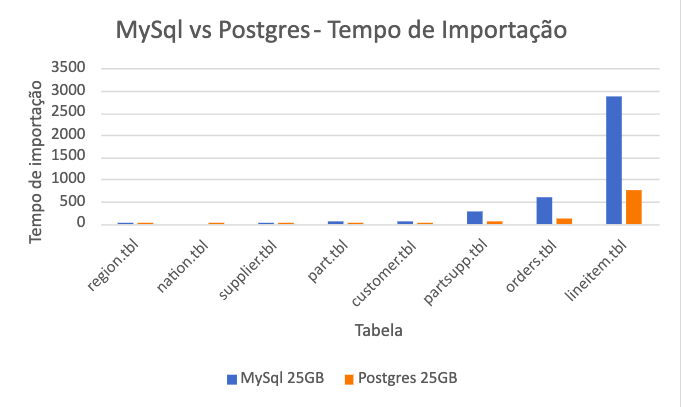
\includegraphics[width=\textwidth]{Graphs/ImportTime.png}\\
  \caption{Gráfico de barras - Tempo de Importação MySQL vs PostgreSQL.}
  \label{fig:row_import_time}
\end{figure}
Analisando o gráfico, o tempo de importação varia significativamente entre as tabelas, principalmente nas últimas três tabelas. A tabela \textit{lineitem} levou o maior tempo para importar, enquanto a tabela \textit{nation} levou o menor tempo para importar.
Isso provavelmente se deve ao fato de que a tabela lineitem.tbl é muito maior do que as outras, tanto em tamanho de ficheiro como em número de linhas.\\
\quad O gráfico também mostra que o tempo de importação é geralmente menor para o PostgreSQL do que para o MySQL. Isso pode ser devido ao fato de que o PostgreSQL é um sistema de base de dados mais eficiente.

\quad Para termos melhores conclusões iremos analisar a relação do tempo de importação de cada tabela nos dois motores de pesquisa com o tamanho do ficheiro.

\quad O gráfico resultante dessa relação é o seguinte:

\begin{figure}[H]
  \centering
  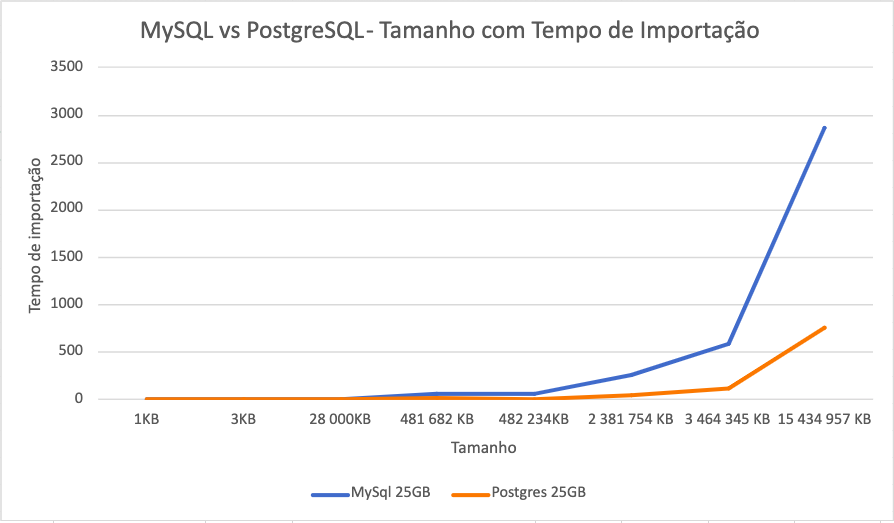
\includegraphics[width=\textwidth]{Graphs/SizevsImport.png}\\
  \caption{Gráfico de barras - Tempo de Importação MySQL vs PostgreSQL em relação ao tamanho.}
  \label{fig:row_import_time2}
\end{figure}


\quad Analisando o gráfico, este demonstra que o tempo de importação aumenta consideravelmente para tabelas maiores, como \textit{lineitem} e \textit{orders}, 15 434 957 KB e 3 464 345 KB, respetivamente. Essa tendência indica que o tamanho dos dados é um fator crucial que influencia o desempenho da importação.\\

\quad O gráfico apresentado revela uma discrepância interessante entre as tabelas \textit{part} e \textit{customer}. Apesar de \textit{customer} ter mais kilobytes (KB), o seu tempo de importação é menor em relação ao \textit{part} em ambos os motores. Essa observação exige uma investigação mais profunda para identificar os fatores que contribuem para essa diferença.\\

\quad Portanto iremos analisar mais um gráfico para verificarmos se o número de linhas influencia.\\

\quad O próximo gráfico mostra a relação do tempo de importação de cada tabela para os motores de pesquisa MySQL e PostgreSQL com o número de linhas de cada tabela.\\


\begin{figure}[H]
  \centering
  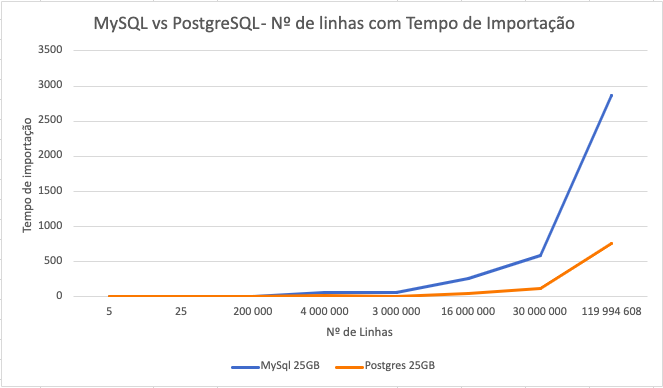
\includegraphics[width=\textwidth]{Graphs/RowsvsImportTime.png}
  \caption{Gráfico de barras - Tempo de Importação MySQL vs PostgreSQL em relação ao número de linhas.}
  \label{fig:row_import_time3}
\end{figure}

\quad Tal como referido anteriormente, a tabela \textit{customer} apresesenta um tempo de importação menor do que \textit{part} em ambos os motores, mesmo com um tamanho de ficheiro ligeiramente maior. Com este gráfico podemos verificar que a causa para tal é o número de linhas ser menor no \textit{customer}. O ficheiro da tabela \textit{part} é maior visto que este apresenta mais uma coluna em relação ao customer, e os tipos de dados são mais compactos no \textit{customer} do que no \textit{part}.\\

\textbf{Observações/Conclusões:}
Os gráficos desta secção forneceram informações valiosas sobre o desempenho de importação de dados nos motores de pesquisa MySQL e PostgreSQL. A análise revela diversos pontos importantes:\\
O PostgreSQL destaca-se como a opção mais rápida para importação de dados em geral. Sua arquitetura otimizada para processamento em massa e operações de importação resulta em tempos de importação menores, especialmente para grandes conjuntos de dados.\\
O tempo de importação varia entre as tabelas, com tabelas maiores geralmente levam mais tempo para serem importadas. Essa observação indica que o tamanho da tabela é um fator crucial que influencia o desempenho da importação. O número de linhas podem influenciar o tempo de importação. Um maior número de linhas aumenta o tempo de processamento.
O tempo de importação no MySQL é cinco vezes superior ao do PostgreSQL.
Com base nas considerações acima, o PostgreSQL é geralmente a melhor escolha para a maioria das aplicações que lidam com grandes volumes de dados ou exigem alto desempenho de importação.

\subsection{Criação das chaves primárias e estrangeiras(PK e FK)}

\quad As chaves primárias e estrangeiras são ferramentas essenciais para garantir a qualidade e confiabilidade dos dados numa base de dados relacional. \\
A chave primária define um identificador único para cada linha da tabela. Essa chave garante que nenhuma linha seja duplicada e facilita a busca e recuperação de dados específicos. A chave estrangeira estabelece uma relação entre duas tabelas, referenciando a chave primária de outra tabela, permitindo que os dados de uma tabela sejam vinculados a dados de outra tabela.\\

\quad Iremos analisar os resultados obtidos na secção \textbf{6.2 Criação das chaves primárias e estrangeiras (PK e FK)}, e os resultados obtidos foram os seguintes:

\begin{figure}[H]
  \centering
  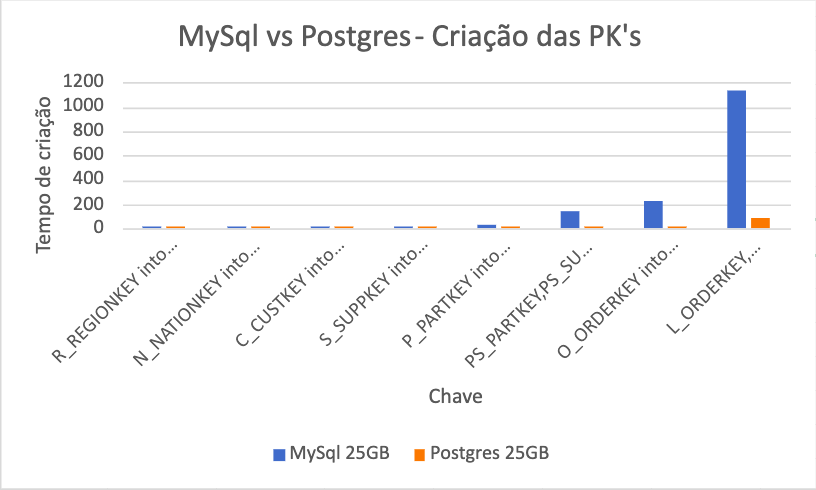
\includegraphics[width=\textwidth]{Graphs/PKCreation.png}
  \caption{Gráfico de barras - Tempo de criação de PK MySQL vs PostgreSQL.}
  \label{fig:PKCreation1}
\end{figure}



\quad Após análise do gráfico e da tabela da secção \textbf{6.2}, podemos tirar conclusões de que o PostgreSQL tem um desempenho muito superior em relação ao MySQL. \\

A diferença fica mais notável, quando as primary keys são colocadas nas tabelas maiores. Ou seja, quanto maior for a tabela, mais é o tempo de criação das chaves primárias.

Para confirmar isso, iremos criar um novo gráfico para sustentar a nossa suposição.

\begin{figure}[H]
  \centering
  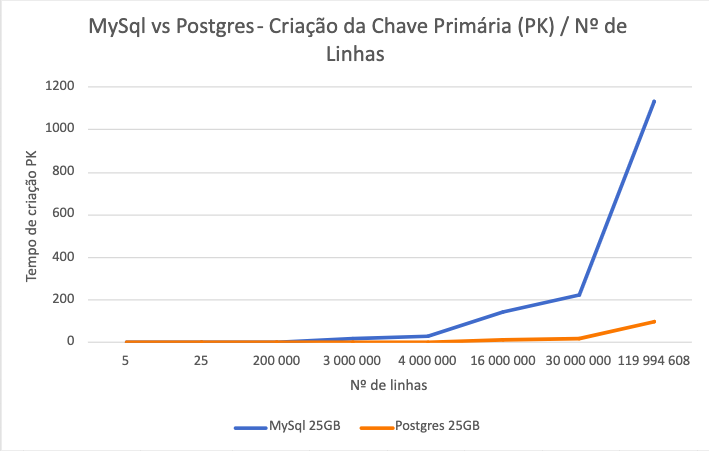
\includegraphics[width=\textwidth]{Graphs/linesvspk.png}
  \caption{Gráfico de barras - Tempo de criação PK MySQL vs PostgreSQL em relação ao número de linhas.}
  \label{fig:PKCreation2}
\end{figure}

\quad Tal como imaginado, quanto mais linhas existirem maior é o tempo de criação de chaves primárias. \\
\quad Podemos concluir que o PostgreSQL geralmente apresenta um desempenho bastante superior em comparação ao MySQL, especialmente me grandes volumes de dados. Essa diferença de performance pode ser atribuída a diversos fatores, como algoritmos otimizados, maior flexibilidade de índices, gestão de memória eficiente e otimização para grandes volumes de dados.\\

\quad O postgreSQL utiliza algoritmos otimizados para criação de indices B-tree, como inserção em massa, balanceamento de B-tree e cache, que otimizam o processo e reduzem o tempo de criação, já o MySQL utiliza algoritmos mais simples para criação de índices, o que pode levar a um desempenho menos eficiente em grandes volumes de dados.\\

\quad O postgreSQL oferece maior flexibilidade na criação de índices, permitindo a utilização de diversos tipos, como hash e parciais, para otimizar consultas específicas. O MySQL possui menos flexibilidade na criação de índices, limitando as opções de otimização para consultas complexas.\\

\quad Iremos abordar a criação de chaves estrangeiras, para avaliarmos qual dos dois motores de busca tem um melhor desempenho na criação destes.\\


\begin{figure}[H]
  \centering
  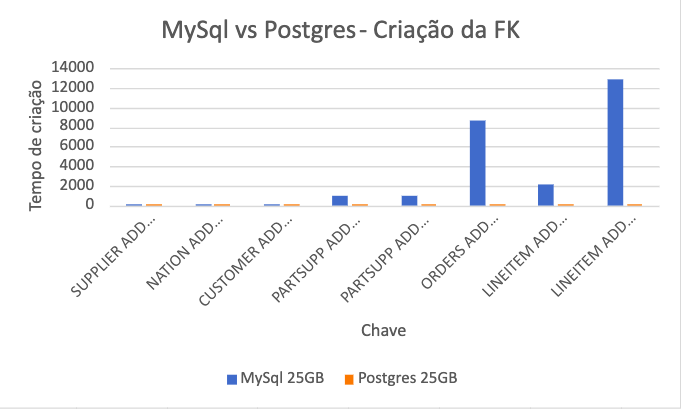
\includegraphics[width=\textwidth]{Graphs/FKCreation.png}
  \caption{Gráfico de barras - Tempo de criação FK MySQL vs PostgreSQL.}
  \label{fig:PKCreation2}
\end{figure}

Analisando a tabela correspondente à criação de chaves estrangeiras, vemos uma discrepância enorme entre o PostgreSQL e o MySQL.\\

Inicialmente, o MySQL e PostgreSQL têm resultados parcialmente iguais, mas quando as chaves estrangeiras são referenciadas a tabelas com um nº de linhas elevado, o MySQL fica com um desempenho muito inferior em relação ao PostgreSQL, sendo que uma das vantagens de usar o MySQL é  ser mais rápido com comandos somente leitura ao custo de simultaneidade, enquanto o PostgreSQL funciona melhor com operações de leitura e gravação, conjuntos de dados massivos e consultas complicadas, por essa razão que o PostgreSQL é mais eficiente.\\

A combinação de algoritmos otimizados, maior flexibilidade de índices, gestão eficiente de referências, otimização para grandes volumes de dados, suporte para multiprocessamento e suporte complexo para cascatas  e restrições de referência torna o PostgreSQL a escolha ideal para aplicações que exigem a criação e gestão de chaves estrangeiras. O MySQL, por outro lado, pode ser uma opção adequada para aplicações com menor volume de dados ou que não exigem um desempenho tao alto na criação de chaves estrangeiras.\\

\clearpage
\subsection{Tempo de execução sem PK's e FK's utilizando 1 thread numa base
de dados de 25GB}

Um dos objetivos do projeto, é analisar o desempenho dos dois motores de pesquisa nas pesquisas sem chaves.

Nesta subsecção iremos comparar o desempenho do MySQL vs PostgreSQL ao executar a mesma pesquisa sem chaves utilizando uma única thread.

Apresentamos agora os tempos de execução sem PK's e FK's utilizando 1 thread.

NOTA: A query 2,17,20,21 não podemos tirar conclusões visto que não deixamos a pesquisa ir até ao fim, visto que passou uma hora e não tivemos nenhum resultado. Destas querys, podemos concluir que na Q19 foi mais rápido no PostgreSQL.
\begin{figure}[H]
  \centering
  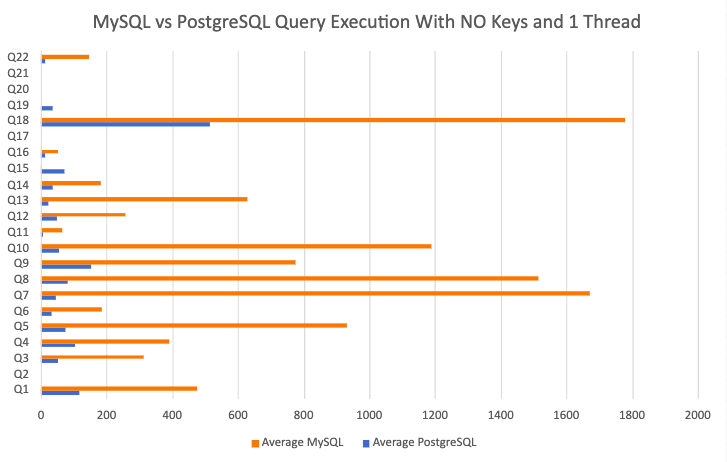
\includegraphics[width=\textwidth]{Graphs/mysqlvspostgres_withoutkeys_onethread.png}
  \caption{Gráfico de barras - MySQL vs PostgreSQL - 1 thread sem chaves.}
  \label{fig:PKCreation2}
\end{figure}

Analisando a tabela correspondente ao tempo de execução sem chaves e com 1 thread, vemos uma grande diferente entre os dois motores de busca.

Há exceção da query 15, o PostgreSQL teve um desempenho absurdamente melhor do que o MySQL.

A partir da tabela, o tempo de execução total da querys MySQL foi \textbf{955,1810096\%} em relação ao PostgreSQL. A query \textbf{Q7} é a query que nos chama mais à atenção, visto que foi a query que demorou mais tanto no PostgreSQL como no MySQL. \\

Esta query é bastante complexa e envolve várias operações que podem ser lentas em grandes volumes de dados.

A subconsulta dentro da claúsula where \textit{'select l\underline{}orderkey from LINEITEM group by l\underline{}orderkey having sum(l\underline{}quantity) \textgreater 314'} é ineficiente visto que a tabela LINEITEM é a maior. Isso ocorre porque a base de dados precisa de calcular a soma para cada l\underline{}orderkey antes de poder filtrar os resultados.

Esta consulta junta três tabelas (customer, orders e lineitem) usando clausulas JOIN. Visto que 2 delas são as maiores e visto que não existe indíces adequados, a junção irá ser demorada. 

 A consulta utiliza a cláusula GROUP BY com funções de agregação (SUM), o que pode ser intensivo em termos de processamento, especialmente quando agrupado por várias colunas.

A cláusula ORDER BY é usada com a função de agregação SUM, o que pode ser custoso em termos de desempenho, pois a base de dados precisa calcular a soma para cada grupo antes de ordenar os resultados.


Em termos de maior diferença entre PostgreSQL com MySQL, a query 8. Neste caso, MySQL é \textbf{3549,631184} \%.  Para termos uma boa conclusão iremos analisar os explains dos dois motores.\\

O MySQL tem um custo total extremamente alto e o PostgreSQL é muito inferior.
No MySQL é utilizado uma operação de junção (nested loop join) entre todas as tabelas. Sendo bastante ineficiente especialmente para grandes volumes de dados, porque cada linha de uma tabela é combinada com todas as linhas das outras tabelas, resultando num grande número de combinações.
No PostgreSQL são utilizadas junções hash paralelas, o que é mais eficiente, especialmente em sistemas com múltiplos núcleos de processamento. Isso ajuda a distribuir a carga de trabalho entre os núcleo de CPU, melhorando o desempenho geral da consulta.
No MySQL, há um grande número de operações de leitura sequencial, o que significa que a base de dados está a percorrer todas as linhas para encontrar os dados necessários. Isso geralmente, é menos eficiente do que usar índices para buscar dados específicos (iremos analisar os indices nas próximas secções).
No PostgreSQL, embora ainda haja operações de leitura sequencial, elas são paralelizadas, o que pode melhorar o desempenho em sistemas com vários núcleos de CPU.
No MySQL é utilizado uma tabela temporária, e uma ordenação em ficheiro (filesort) o que pode indicar que a base de dados teve que usar recursos adicionais para manipular os resultados intermediários da consulta.

De uma forma geral, o PostgreSQL apresenta melhores resultados e mais eficientes principalmente quando não existem chaves e só é utilizado uma thread.

\clearpage
\subsection{Tempo de execução sem PK's e FK's utilizando 5 thread's numa base
de dados de 25GB}


Nesta subsecção iremos comparar o desempenho do MySQL vs PostgreSQL ao executar a mesma pesquisa sem chaves utilizando 5 thread, para que possamos verificar se as thredas têm algum impacto quando não são usadas chaves.

Apresentamos agora os tempos de execução sem PK's e FK's utilizando 5 thread.

NOTA: A query 2,17,19,20,21 não podemos tirar conclusões visto que não deixamos a pesquisa ir até ao fim, visto que passou uma hora e não tivemos nenhum resultado. Destas querys, podemos concluir que na Q19 foi mais rápido no PostgreSQL.

Apresentamos agora os tempos de execução sem PK's e FK's utilizando 5 thread's.
\begin{figure}[H]
  \centering
  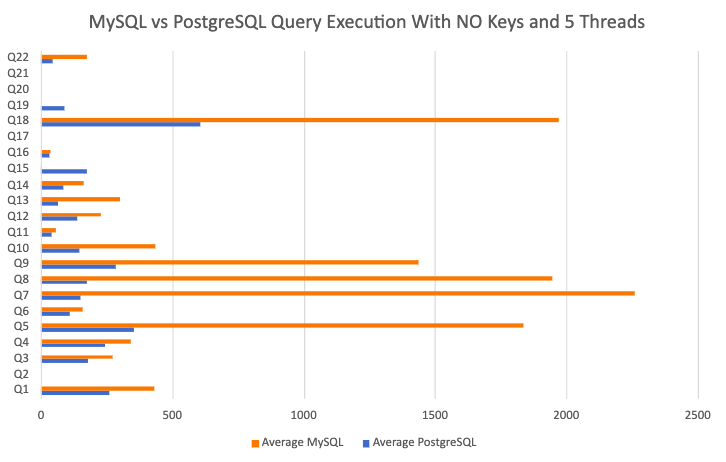
\includegraphics[width=\textwidth]{Graphs/mysqlvspostgres_withoutkeys_fivethreads.png}
  \caption{Gráfico de barras - MySQL vs PostgreSQL - 5 thread's sem chaves.}
  \label{fig:PKCreation2}
\end{figure}

Tal como no gráfico anterior, o resultado global dá nos novamente o postgreSQL como o melhor motor de pesquisa para as pesquisas sem chaves e com 5 threads.

Apesar disso, o tempo de execução total da querys MySQL foi \textbf{272,1583536\%} em relação ao PostgreSQL, o que diminuiu bastante em relação ao uso de apenas uma thread.

Em comparação com o gráfico da subsecção anterior, os tempos de execução aumentaram,
visto que são usadas 5 threads, em que têm de dividir os recursos tais como memória e etc. Portanto
o tempo de pesquisa seria relativamente mais alto, tal como esperado.

Visto que na secção anterior analisamos a query \textbf{Q7}, e mesmo assim é a que tem maior diferença entre mysql e postgres, iremos analisar a \textbf{Q8}, que é a segunda com maior diferença.

O MySQL usa uma estratégia de hash join, o que significa que ele une tabelas repetidamente com base em colunas específicas.
Ele executa uma varredura completa em muitas tabelas, incluindo tabelas grandes, como pedidos e itens de linha.
Isto pode ser muito caro para processar grandes conjuntos de dados.
A classificação é feita nos resultados intermediários antes do agrupamento, o que adiciona outra camada de custo.


PostgreSQL usa uma abordagem de coleta para agregação.
Primeiro ele filtra e une tabelas menores, como região e nação.
Em seguida, ele usa processamento paralelo para digitalizar e unir tabelas maiores, como pedidos e itens de linha.
Por fim, agrupa os dados por ano extraídos da colunaorders.o\underline{}orderdate.

Para conjuntos de dados muito grandes, a abordagem de fusão e coleta do PostgreSQL com processamento paralelo é mais eficiente.


Iremos abordar a \textbf{Q16}, para analisarmos a razão pela qual os tempos são parecidos.

Após verificarmos o custo estimado notamos uma diferença enorme, mas os resultados são praticamente os mesmos, tornando o mysql como mais rápido.

PostgreSQL usa uma estratégia de coleta e mesclagem para agregação.

Filtra e junta tabelas menores primeiro (como na subconsulta2 para fornecedores com reclamações).
Usa processamento paralelo para digitalizar e unir tabelas maiores (part e partsupp).
Classifica os resultados por diversas colunas (p\underline{}brand, p\underline{}type e p\underline{}size) e depois os agrega usando count(DISTINCT partsupp.ps\underline{}suppkey).


MySQL usa uma série de hash joins em todo o plano.
Executa inicialmente uma varredura completa da tabela no partsupp.
Usa uma subconsulta para filtrar peças com base em critérios específicos (p\underline{}brand, p\underline{}type e p\underline{}size).
Classifica e agrupa os resultados finalmente.

O PostgreSQL parece mais adequado para cenários com tabelas grandes como o partsupp. O processamento paralelo ajuda a distribuir a carga de trabalho entre vários threads, melhorando potencialmente o desempenho.
O MySQL pode ser a escolha do otimizador para consultas de agregação mais simples, sem condições de filtragem complexas.

Portanto, após analisarmos os resultados, notamos que o uso de threads piora o tempo de execução de querys.

Iremos apresentar noutra secção a diferença com uso de 1 thread vs 5 threads entre motores de pesquisa.

Concluindo, o PostgreSQL é superior ao MySQL quando são executadas 5 threads e não existem chaves.

\clearpage
  \subsection{Comparação da média do tempo de execução sem PK's e FK's
  utilizando 1 vs 5 thread numa base de dados de 25.(MySQL, PostgreSQL)}
  
  \quad Nesta subsecção iremos comparar o desempenho do MySQL ao executar a mesma consulta com diferentes números de threads, especificamente 1 e 5 threads, sem chaves. 
  
  O objetivo é avaliar o impacto do paralelismo na eficiência da consulta e determinar se o aumento de threads resulta numa melhoria significativa no tempo de resposta.\\
  
  Também iremos fazer uma analise ao desempenho do postgreSQL ao executar a mesma consulta com diferentes números de threads.

  \begin{figure}[H]
    \centering
    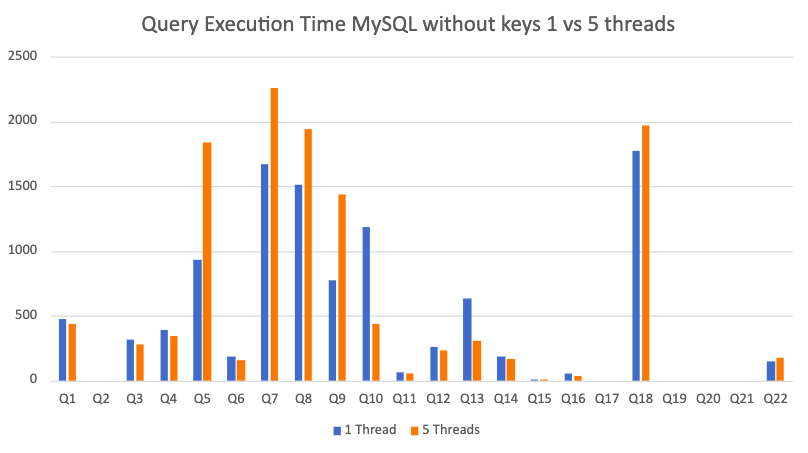
\includegraphics[width=\textwidth]{Graphs/mysql_withoutkeys_1vs5threads.png}
    \caption{Gráfico de barras - MySQL - 1 vs 5 thread sem chaves.} 
    \label{fig:PKCreation2}
  \end{figure}
  
  As querys 2,17,19,20,21 não irão ser analisadas visto que nem com 1 thread nem 5 threads estas foram executadas até ao fim.

  Apartir da tabela e do gráfico apresentado, 9 das 17 que observamos são mais rápidas nas 5 threads.

  Sendo que podemos analisar que essas 9 são nas querys mais simples e que de forma geral demoram menos tempo, sendo que nessas querys a diferença entre 1 thread e 5 thread é pequena. \\

  Já quando analisamos as outro 8 queryes estas já são mais complexas que têm mais junções e combinações a fazer, tornando assim o uso de apenas uma thread um benefício.

  Portanto neste gráfico é 50\%/50\%, depende bastante do objetivo do projeto, se as querys forem mais simples o uso de 5 threads é uma vantagem, torna a execução mais rápida e são executadas mais querys ao mesmo tempo.



  \begin{figure}[H]
    \centering
    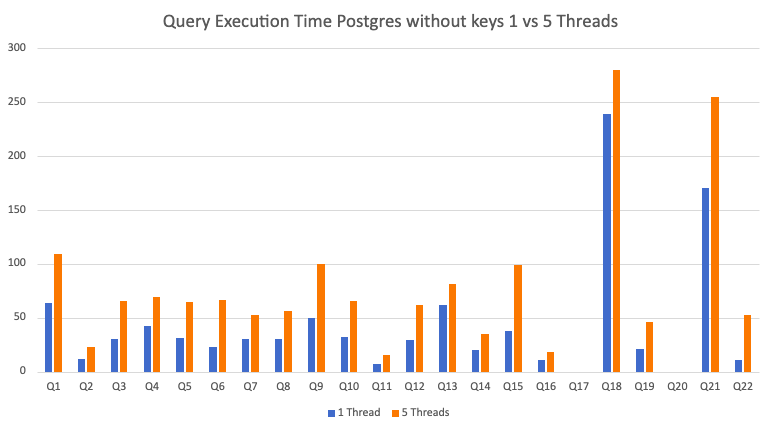
\includegraphics[width=\textwidth]{Graphs/postgres_withoutkeys_1vs5.png}
    \caption{Gráfico de barras - PostgreSQL - 1 vs 5 thread sem chaves.} 
    \label{fig:PKCreation2}
  \end{figure}

  Com base nas tabelas acima referidas e no gráfico mostrado, podemos verificar que 100\% das querys são mais rápidas quando são usadas 
  
  Uma das teorias para tal, é as querys estarem a dividir recursos entre si, tendo assim menos desempenho quando começam a executar. Iremos abordar agora uma possível explicação entre as diferenças entre mysql que teve 50\% de sucesso 1 thread e o postgres que teve 100\% de sucesso com 1 thread.

  O otimizador do MySQL pode escolher planos de execução menos eficientes para determinadas consultas, levando a um desempenho mais lento com vários threads. Isso pode ser devido a fatores como estratégia de junção, otimização de subconsulta ou padrões de acesso a dados. Em algumas consultas MySQL, uma única operação de junção pode ser o gargalo de desempenho. Mesmo com a paralelização, outros estágios podem ter que aguardar a conclusão dessa junção, limitando o benefício de vários threads, e adicionar mais threads pode não melhorar o desempenho. Isto pode ser especialmente verdadeiro para consultas que envolvem a leitura de grandes quantidades de dados do disco.

  A implementação de threading do PostgreSQL pode ser mais eficiente em determinados cenários em comparação com o MySQL. Poderia ter melhor agendamento de threads, mecanismos de sincronização ou técnicas de gestão de memória.

  O otimizador de consultas do PostgreSQL pode ser mais conservador em sua estimativa dos benefícios da paralelização. Poderia favorecer planos mais simples de thread único para evitar sobrecarga potencial ou degradação de desempenho.






\clearpage
\subsection{Tempo de execução com PK's e FK's utilizando 1 thread numa base
de dados de 25GB}
Um dos objetivos do projeto, é analisar o desempenho dos dois motores de pesquisa nas pesquisas com chaves.

Nesta subsecção iremos comparar o desempenho do MySQL vs PostgreSQL ao executar a mesma pesquisa com chaves utilizando uma única thread.


NOTA: A query 17,20,21 não podemos tirar conclusões visto que não deixamos a pesquisa ir até ao fim, visto que passou uma hora e não tivemos nenhum resultado. Destas querys, podemos concluir que a Q17 e Q20 foi mais rápida no MySQL.


Apresentamos agora os tempos de execução com PK's e FK's utilizando 1 thread.
\begin{figure}[H]
  \centering
  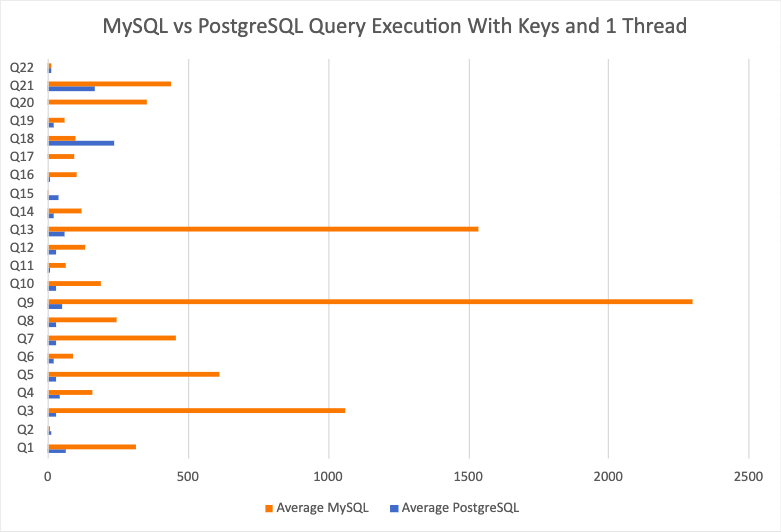
\includegraphics[width=\textwidth]{Graphs/mysqlvspostgresql_withkeys_onethread.png}
  \caption{Gráfico de barras - MySQL vs PostgreSQL - 1 thread com chaves.}
  \label{fig:PKCreation2}
\end{figure}
\quad Com base nesta comparação, pode-se observar que em muitos casos o postgreSQL apresenta tempos de execução significativamente mais baixos do que MySQL para as consultas do TPC-H.

Isso pode ser atríbuido a várias razões incluindo, \textit{Otimizações do PostgreSQL} o postgreSQL é conhecido por ter um otimizador de consulta sofisticado que pode gerar planos de execução eficientes para consultas complexas. Isso pode resultar em tempos de execução mais rápidos para consutlas específicas em comparação com o MySQL, \textit{Arquitetura do PostgreSQL} o postgreSQL tem uma arquitetura robusta que suporta recursos avançados, como suporte a vários tipos de índices, sendo que esses recursos podem contribuir para um desempenho melhor em cenários de consulta intensiva, como o TPC-H.

Tal como referido anteriorment, o otimizador do MySQL pode escolher planos de execução menos eficientes para determinadas consultas, levando a um desempenho mais lento com vários threads. Isso pode ser devido a fatores como estratégia de junção, otimização de subconsulta ou padrões de acesso a dados. 


\quad Mas existem algumas exceções, tais como a query 17,18,20,21.

Consultas como Q2, Q6, Q8, Q11 e Q15 são menos complexas, envolvem menos junções ou operações mais simples.
Para essas consultas menos complexas, o PostgreSQL também tende a ter tempos de execução mais baixos em comparação com o MySQL na maioria dos casos.

Podendo concluir, que o PostgreSQL quando utilizado 1 thread e chaves é muito mais eficiente, principalmente quando envolve pesquisas mais complexas e mais demoradas.

\clearpage
\subsection{Tempo de execução com PK's e FK's utilizando 5 thread's numa base
de dados de 25GB}

Um dos objetivos do projeto, é analisar o desempenho dos dois motores de pesquisa nas pesquisas com chaves.

Nesta subsecção iremos comparar o desempenho do MySQL vs PostgreSQL ao executar a mesma pesquisa com chaves utilizando uma 5 threads, com objetivo de analisar se o aumento do número de threads tem algum impacto no desempenho.


NOTA: A query 17,20,21 não podemos tirar conclusões visto que não deixamos a pesquisa ir até ao fim, visto que passou uma hora e não tivemos nenhum resultado. Destas querys, podemos concluir que na Q20 foi mais rápida no PostgreSQL.



Apresentamos agora os tempos de execução com PK's e FK's utilizando 5 thread.
\begin{figure}[H]
  \centering
  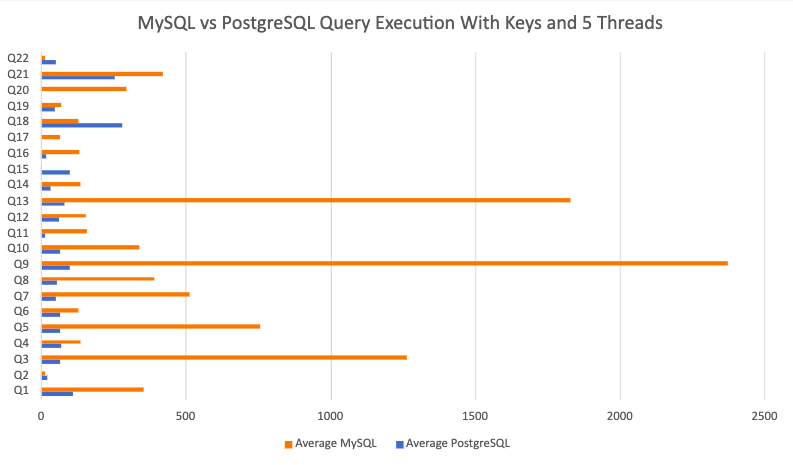
\includegraphics[width=\textwidth]{Graphs/mysqlvspostgres_withkeys_fivethreads.png}
  \caption{Gráfico de barras - MySQL vs PostgreSQL - 5 thread com chaves.}
  \label{fig:PKCreation2}
\end{figure}


\quad Apartir deste gráfico podemos concluir o mesmo que na subsecção anterior. O postgreSQL apresenta tempos de execução significativamente mais baixos do que MySQL, menos nas query 2,15,16,17,18,20,21.
\quad Em comparação com o gráfico da subsecção anterior, os tempos de execução aumentaram, visto que são usadas 5 threads, em que têm de dividir os recursos tais como memória e pelas razões escritas na secção \textbf{7.5}, da figura 5. 

\quad Em relação à secção \textbf{7.6}, os resultados do PostgreSQL são drásticamente piores, apesar disso o PostgreSQL tem uma grande vantagem, visto que o tempo de execução total do mysql é \textbf{576,2615614\%} superior em relação ao PostgreSQL.

Concluindo, o PostgreSQL é superior em relação ao MySQL com uso de chaves e com 5 threads.
\clearpage
  \subsection{Comparação da média do tempo de execução com PK's e FK's
  utilizando 1 vs 5 thread numa base de dados de 25.(MySQL, PostgreSQL)}
  
  \quad Nesta subsecção iremos comparar o desempenho do MySQL ao executar a mesma consulta com diferentes números de threads, especificamente 1 e 5 threads. 
  
  O objetivo é avaliar o impacto do paralelismo na eficiência da consulta e determinar se o aumento do número de threads resulta numa melhoria significativa no tempo de resposta.\\

  Também iremos fazer uma analise ao desempenho do postgreSQL ao executar a mesma consulta com diferentes números de threads.

  \begin{figure}[H]
    \centering
    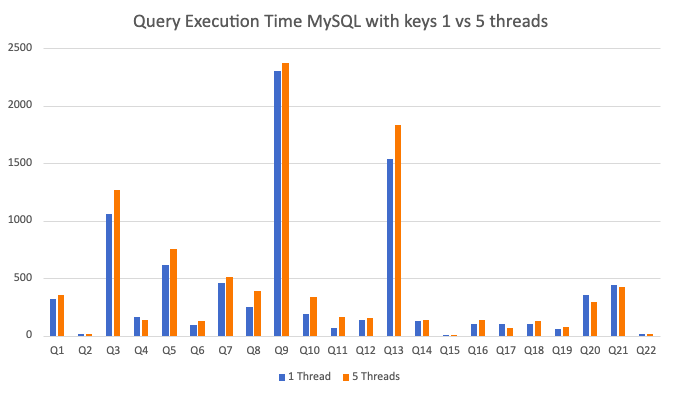
\includegraphics[width=\textwidth]{Graphs/mysql_withkeys_1vs5threads.png}
    \caption{Gráfico de barras - MySQL - 1 vs 5 thread com chaves.} 
    \label{fig:PKCreation2}

  \end{figure}

  \quad É possível analisar que a média dos tempos é sempre mais baixa quando estes são executados com apenas uma thread, o que já era algo de esperar. Iremos dar uma explicação após mostrarmos a comparação para o PostgreSQL, que na teoria também será menor para as execuções de 1 thread.
    
  Neste caso, 17 das 22 querys são mais rápidas quando usadas 1 threads, em comparação aos tempos de execução sem chaves existe uma boa diferença, visto que com chaves a utilização de 1 thread é mais benéfico do que com 5 threads. Já sem chaves é benéfico utilizar 1 thread quando as querys são mais complexas. Neste caso em que é utilizado chaves, é mais vantajoso utilizar 1 thread que 5.

  Mesmo assim, os resultados são bastante parecidos, sendo que o MySQL de forma geral é bom tanto com 1 thread como com 5 threads(principalmente quando são mais simples).

  \begin{figure}[H]
    \centering
    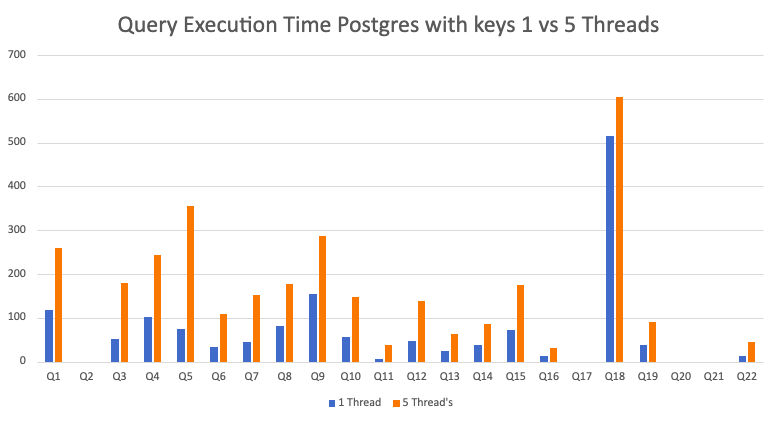
\includegraphics[width=\textwidth]{Graphs/postgres_withkeys_1vs5.png}
    \caption{Gráfico de barras - PostgreSQL - 1 vs 5 thread com chaves.} 
    \label{fig:PKCreation2}
  \end{figure}

  NOTA: Não iremos tirar conclusões acerca da query 2,17,20 e 21 (Não temos dados para analisar).

Analisando o resultado, as execuções com 1 thread são as mais rápidas, o otimizador de consultas de PostgreSQL pode ser mais conservador na sua estimativa dos benefícios da paralelização. Sendo que pode favorecer planos mais simples de uma única thread para evitar sobrecarga potencial ou degradação de desempenho.
  
  
  
\quad As consultas simultâneas podem competir por recursos partilhados, especialmente se as consultas estiverem a tentar aceder aos mesmos recursos ao mesmo tempo.
O uso de várias threads pode aumentar o overhead do sistema devido à criação e gestão de threads adicionais. Isso pode consumir recursos do sistema, como CPU e memória, reduzindo a eficiência geral. 
Dependendo da natureza das consultas e da carga de trabalho, várias consultas simultâneas podem sobrecarregar o sistema de base de dados, levando a latências mais altas e tempos de resposta mais lentos. 
 




\clearpage
\subsection{Comparação da média do tempo de execução entre com chaves vs sem chaves numa base de dados de 25GB PostgreSQL}
Nesta secção, vamos analisar a comparação da média do tempo de execução entre consultas com e sem chaves numa base de dados PostgreSQL utilizando diferentes números de threads, a primeira é com 1 thread e depois analisamos com 5 threads.

O objetivo é avaliar o impacto da presença de chaves primárias no desempenho de consultas complexas.

NOTA: A query 2 e 21, apesar de não termos deixado a pesquisa sem chaves ir até ao fim, podemos concluir que foram mais rápido na pesquisa com chaves, visto que demorou 1 hora e ainda não tinhamos o resultado. A query 17 e 20 não podemos ter conclusões, passado uma hora não tinhamos resultados nem na pesquisa com chaves nem sem chaves.


\begin{figure}[H]
  \centering
  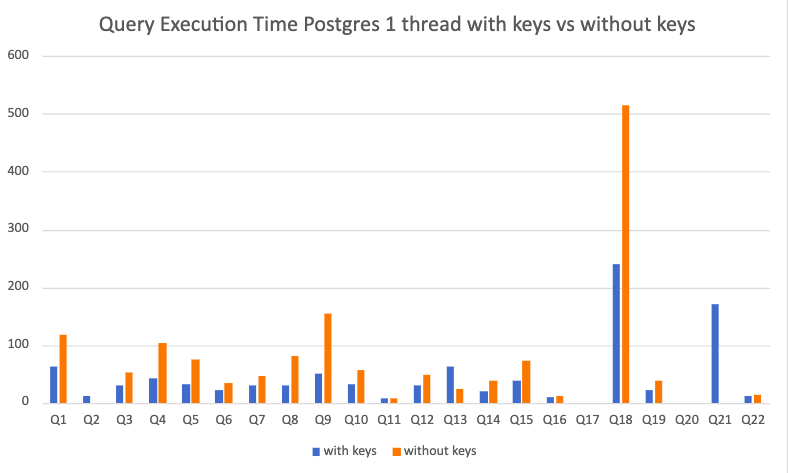
\includegraphics[width=\textwidth]{Graphs/postgres1thread_withkeysvswithoutkeys.png}
  \caption{Gráfico de barras - PostgreSQL - with keys vs without keys utilizando 1 thread.} 
  \label{fig:PKCreation2}
\end{figure}


Analisando o gráfico de barras disponibilizado, 17 das 18 querys possíveis de análise são mais rápidas quando ocorre o uso das chaves.

A query 13 ficou notável que é mais eficiente sem o uso de chaves, iremos analizar os explain tirando conclusões acerca das razões para tal.

Com Chaves usa uma "varredura apenas de índice paralelo usando customer\underline{}pkey no cliente". Isso indica acesso eficiente à tabela de clientes aproveitando o índice de chave primária (customer\underline{}pkey). Geralmente, isso é mais rápido do que verificar a tabela inteira.
Sem chaves usa um "Parallel Seq Scan on customer". Isso sugere uma varredura completa da tabela do cliente, potencialmente acessando mais dados do que o necessário.

Uma vantagem do plano com chaves: Acesso mais rápido aos dados do cliente usando o índice de chave primária.

Ambos os planos: utilizam um "Parallel Hash Left Join" para combinar dados das tabelas de clientes e pedidos com base na coluna c\underline{}custkey. As estimativas de custos para a operação de junção são muito semelhantes em ambos os planos.

Uma razão pela qual é mais rápido sem uso de chaves são as seguintes:\\
Quando uma grande parte da tabela precisa ser acedida, um full scan pode ser mais rápido do que usar índices. Isso ocorre porque o custo de aceder os blocos de dados diretamente pode ser menor do que o custo de percorrer a estrutura do índice, e em seguida, aceder os dados correspondentes.
Evitar o uso de chaves pode reduzir a sobrecarga à manutenção dessas estruturas. Em consultas que retornam a maioria dos registos da tabela, o benefício de usar um índice para localizar os registos pode ser superado pelo custo adicional de manter e usa esse índice.
Se a consulta fosse mais seletiva, o uso de chaves seria mais benéfico e o resultado seria mais eficiente e rápido.

Apresentamos um gráfico com a mesma ideia mas com a utilização de 5 threads.

\begin{figure}[H]
  \centering
  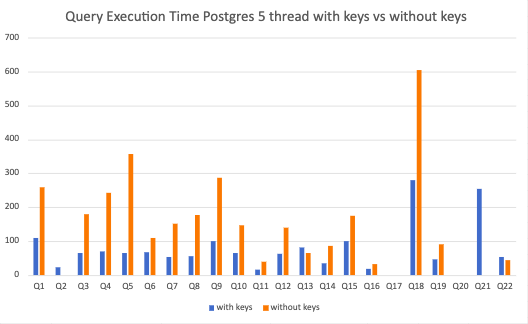
\includegraphics[width=\textwidth]{Graphs/postgres5threads_withkeysvswithoutkeys.png}
  \caption{Gráfico de barras - PostgreSQL - with keys vs without keys utilizando 5 thread.} 
  \label{fig:PKCreation2}
\end{figure}
As conclusões que tiramos acima são exatamente iguais. O único dado que podemos adicionar é que com o uso de 5 threads, todas as pesquisas ficaram mais lentas. E à exceção da query \textbf{Q13}, o uso de chaves é benéfico.

\clearpage


\subsection{Comparação da média do tempo de execução entre com chaves vs sem chaves numa base de dados de 25GB MySQL}

Nesta secção, vamos analisar a comparação da média do tempo de execução entre consultas com e sem chaves numa base de dados MySQL utilizando diferentes números de threads, a primeira é com 1 thread e depois analisamos com 5 threads.

O objetivo é avaliar o impacto da presença de chaves primárias no desempenho de consultas complexas.

NOTA: A query 2,17,19,20, apesar de não termos deixado a pesquisa sem chaves ir até ao fim, podemos concluir que foram mais rápido na pesquisa com chaves, visto que demorou 1 hora e ainda não tinhamos o resultado.


\begin{figure}[H]
  \centering
  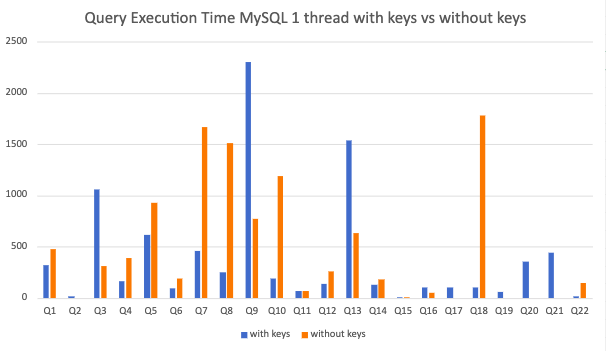
\includegraphics[width=\textwidth]{Graphs/mysqlonethread_withkeysvswithoutkeys.png}
  \caption{Gráfico de barras - MySQL - with keys vs without keys utilizando 1 thread.} 
  \label{fig:PKCreation2}
\end{figure}
Os dados são bastante semelhantes aos do postgres, à exceção da query \textbf{Q3},\textbf{Q9},\textbf{Q17} e \textbf{Q16}

Iremos analisar mais detalhadamente a query \textbf{Q3}.

\textbf{Com chaves} ,  a tabela ORDERS é acedida usando um índice (ref) na coluna O\underline{}CUSTKEY, enquanto no \textbf{sem chaves} é acessada através de uma varredura completa . Dependendo da distribuição dos dados e da eficiência do índice, a varredura completa pode ser mais rápida para aceder uma grande parte da tabela em comparação com a utilização de índices, especialmente se o índice não estiver bem ajustado ou se o custo de acesso ao índice for alto.

Ambos os planos envolvem operações de junção, mas o custo dessas operações pode variar dependendo dos métodos de acesso às tabelas e das condições de junção. No \textbf{com chaves} , a junção entre as tabelas ORDERS e LINEITEM é realizada através de referências a chaves primárias, o que pode introduzir um custo adicional de acesso ao índice. Isso pode contribuir para o aumento do tempo de execução.

Ambos os planos envolvem filtros de dados (attached\underline{}condition) aplicados às tabelas ORDERS e LINEITEM. No entanto, o custo dessas operações de filtragem pode variar dependendo do método de acesso às tabelas e do número de registros que atendem aos critérios de filtragem.

Uma das razões pelas quais o \textbf{com chaves} é mais lento do que \textbf{sem chaves} é que as chaves utilizadas não são muito seletivos para os critérios de filtragem aplicados, o que significa que eles não reduzem eficientemente o número de linhas a serem acedidas. Tornando assim mais leituras de disco e operações de acesso à memória, tornando a consulta mais lenta.



\begin{figure}[H]
  \centering
  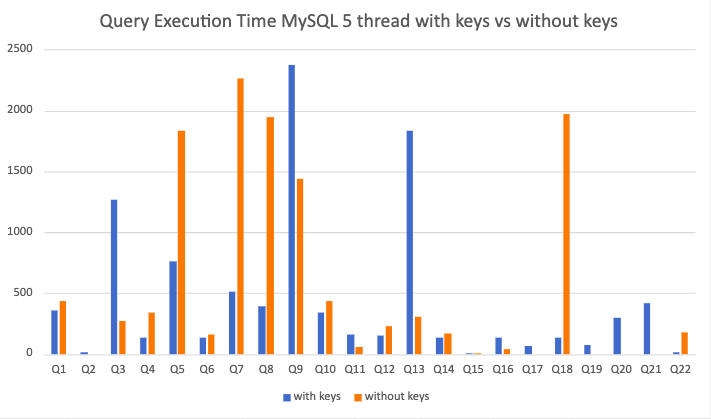
\includegraphics[width=\textwidth]{Graphs/mysql5threads_withkeys_withoutkeys.png}
  \caption{Gráfico de barras - MySQL - with keys vs without keys utilizando 5 thread.} 
  \label{fig:PKCreation2}
\end{figure}

Analisando os resultados, estes são parecidos aos apresentados anteriormente, conseguimos visualizar, que o uso de threads tem um impacto mais negativo quando são usadas chaves do que quando não são usadas as chaves. Nota-se a diferença na query 11 que nem é muito complexa mas que com o uso de threads colocou o dobro mais lenta que anteriormente.

Concluindo, o uso de chaves de forma geral, é mais benéfica isto quando os dados são mais seletivos. Quando os dados não são seletivos e as bases de dados são mais complexas e com um tamanho razoavelmente grande, é preferível não utilizar chaves, visto que o custo de full scan é inferior ao custo de manter um índice e de o utilizar.
\clearpage
\subsection{Comparação média do tempo de execução 1 vs 5 threads com chaves base de dados 40GB(PostgreSQL)}

A nossa primeira base de dados continha cerca de 40GB de dados, executamos as pesquisas para o PostgreSQL com sucesso, mas quando fomos executar no MySQL demoravam imenso tempo, o que nos fez parar. Mas iremos apresentar os resultados e fazer uma comparação no motor de pesquisa PostgreSQL com uma execução com 1 vs 5 threads, e visualizar qual é a mais rápida e mais eficiente.

\begin{figure}[H]
  \centering
  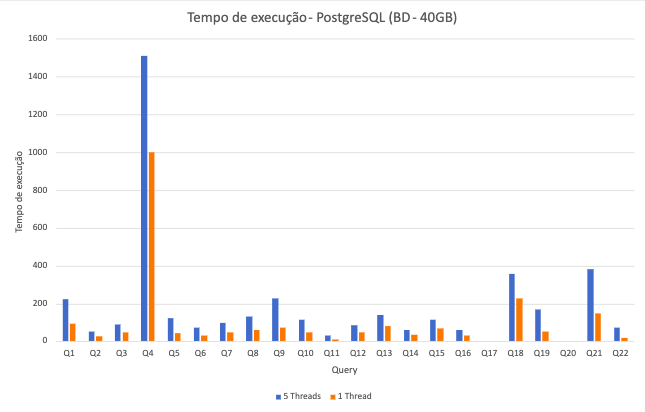
\includegraphics[width=\textwidth]{Graphs/postgresql40gb.png}
  \caption{Gráfico de barras - PostgreSQL - 1 vs 5 thread com chaves (40GB).} 
  \label{fig:PKCreation2}
\end{figure}

Analisando o gráfico, podemos concluir que é mais rápido e eficiente quando é executada apenas uma thread, a razão pela qual isso acontece já referimos antes, com 5 threads estas têm de partilhar o mesmo recurso, ou seja, dividir tornando assim a performance global mais lenta, e outras razões que já referimos desde o ínicio do relatório. 

\clearpage
\subsection{Análise de Explain Plan Rápida vs Query Lenta}
\subsubsection{PostgreSQL - Rápida}
Para a query rápida do PostgreSQL opatamos pela query 11, visto que dos resultados que obtemos foi sempre a mais rápida.\\

Este explian plain é sem uso de chaves.

\begin{lstlisting}[language=SQL]
Sort  (cost=1033765.57..1034180.67 rows=166041 width=36)
  Sort Key: (sum((partsupp.ps_supplycost * (partsupp.ps_availqty)::numeric))) DESC
  InitPlan 1 (returns $1)
    ->  Finalize Aggregate  (cost=454267.05..454267.06 rows=1 width=32)
          ->  Gather  (cost=454266.82..454267.03 rows=2 width=32)
                Workers Planned: 2
                ->  Partial Aggregate  (cost=453266.82..453266.83 rows=1 width=32)
                      ->  Parallel Hash Join  (cost=5705.15..451266.82 rows=266667 width=10)
                            Hash Cond: (partsupp_1.ps_suppkey = supplier_1.s_suppkey)
                            ->  Parallel Seq Scan on partsupp partsupp_1  
                                    (cost=0.00..419450.67 rows=6666667 width=14)
                            ->  Parallel Hash (cost=5663.49..5663.49 rows=3333 width=4)
                                  ->  Hash Join  (cost=1.32..5663.49 rows=3333 width=4)
                                        Hash Cond: (supplier_1.s_nationkey = 
                                            nation_1.n_nationkey)
                                        ->  Parallel Seq Scan on supplier supplier_1  (cost=0.00..5316.33 rows=83333 width=8)
                                        ->  Hash  (cost=1.31..1.31 rows=1 width=4)
                                              ->  Seq Scan on nation nation_1  (cost=0.00..1.31 rows=1 width=4)
                                                Filter: (n_name = 'MOZAMBIQUE'::bpchar)
  ->  Finalize GroupAggregate  (cost=480860.28..560558.78 rows=166041 width=36)
        Group Key: partsupp.ps_partkey
        Filter: (sum((partsupp.ps_supplycost * (partsupp.ps_availqty)::numeric)) > $1)
        ->  Gather Merge  (cost=480860.28..549086.93 rows=533334 width=36)
              Workers Planned: 2
              ->  Partial GroupAggregate  (cost=479860.25..486526.93 rows=266667 
                    width=36)
                    Group Key: partsupp.ps_partkey
                    ->  Sort  (cost=479860.25..480526.92 rows=266667 width=14)
                          Sort Key: partsupp.ps_partkey
                          ->  Parallel Hash Join  (cost=5705.15..451266.82 rows=266667 width=14)
                                Hash Cond: (partsupp.ps_suppkey = supplier.s_suppkey)
                                ->  Parallel Seq Scan on partsupp  
                                    (cost=0.00..419450.67 rows=6666667 width=18)
                                ->  Parallel Hash  (cost=5663.49..5663.49 rows=3333 width=4)
                                      ->  Hash Join  (cost=1.32..5663.49 rows=3333 width=4)
                                            Hash Cond: (supplier.s_nationkey = 
                                            nation.n_nationkey)
                                            ->  Parallel Seq Scan on supplier  (cost=0.00..5316.33 rows=83333 width=8)
                                            ->  Hash  (cost=1.31..1.31 rows=1 width=4)
                                                  ->  Seq Scan on nation  (cost=0.00..1.31 rows=1 width=4)
                                                    Filter: (n_name ='MOZAMBIQUE'::bpchar)

\end{lstlisting}

\textbf{Explicação}\\
Este plano de execução está relacionado a uma consulta que envolve operações de agregação, junção e filtragem.

Inicialmente, ocorre o initplan e finalize aggregate, são etapas preliminares para calcular a soma ponderada dos custos de suplimentos multiplicados pela quantidade disponivel para os produtos. Estes estão relacionados à função de agregação sum usada na consulta.

Posteriormente, uma junção entre tabelas é realizada usando o campo \textit{ps\underline{}suppkey}. Esta é uma junção do tipo hash, que é uma técnica eficiente para unir grandes conjuntos de dados. Ambas as tabelas vão ser acedidas em paralelo. 

Depois, um escaneamento sequencial paralelo é realizado na tabela \textit{partsuup\underline{}1}. Isso é feito para realizar uma junção com a tabela \textit{s\underline{}1}.

Um filtro é aplicado na tabela \textit{nation\underline{}1} para selecionar apenas as linhas onde o país é MOZAMBIQUE.

Os resultados da junção e da agregação são finalizados e os resultados são agrupados pela chave ps\underline{}partkey.

Um filtro é aplicado nos resultados agrupados para selecionar apenas os grupos onde a soma ponderada dos custos de suplimentos multiplicados pela quantidade disponivel é maior que um valor específico. Este valor é calculado na etapa InitPlan.

No final, os resultados finais são classificados em ordem decrescente com base na soma ponderada calculada na etapa initplan.

\subsubsection{PostgreSQL - Lenta}
Uma das querys mais lentas é a query 18, tinhamos outras tais como o 17 e 20, mas visto que dessas 2 não as deixamos ir até ao fim, achamos que as conclusões acerca desta poderão ser mais positivas.

Não está bem formatado, para visualizar melhor recomendamos ver os ficheiros que submetemos com os explain plan.

\begin{lstlisting}[language=SQL]
  
Limit  (cost=13274145.32..13274148.32 rows=100 width=71)
 ->  GroupAggregate  (cost=13274145.32..13291299.74 rows=571814 width=71)
      Group Key: orders.o_totalprice, orders.o_orderdate,
         customer.c_name, customer.c_custkey, orders.o_orderkey
       ->  Sort  (cost=13274145.32..13275574.86 rows=571814 width=44)
            Sort Key: orders.o_totalprice DESC, orders.o_orderdate, 
                customer.c_name, customer.c_custkey, orders.o_orderkey
              ->  Hash Join  (cost=8090754.07..13201874.07 rows=571814 
                                                    width=44)
                   Hash Cond: (lineitem.l_orderkey = orders.o_orderkey)
                    ->  Seq Scan on lineitem  (cost=0.00..3482341.08 
                            rows=119994608 width=9)
                     ->  Hash  (cost=8087710.07..8087710.07 rows=142960 width=43)
                        ->  Hash Join  (cost=6806016.96..8087710.07 
                          rows=142960 width=43)
                              Hash Cond: (orders.o_custkey = customer.c_custkey)
                               ->  Hash Join  (cost=6648545.96..7908660.97 rows=142960
                                           width=24)
                                    Hash Cond: (orders.o_orderkey = lineitem_1.l_orderkey)
                                      ->  Seq Scan on orders  (cost=0.00..829242.00 
                                      rows=30000000 width=20)
                                      ->  Hash  (cost=6646199.96..6646199.96 
                                      rows=142960
                                                         width=4)
                                          ->  Finalize GroupAggregate  
          (cost=6531824.71..6644770.36 rows=142960 width=4)
                                                Group Key: lineitem_1.l_orderkey
                                                 Filter: 
(sum(lineitem_1.l_quantity) > '314'::numeric)
                                                 ->  Gather Merge  
(cost=6531824.71..6631903.93rows=857762 width=36)
                                                       Workers Planned: 2
                                                        ->  Sort  
(cost=6530824.69..6531896.89 rows=428881 width=36)
                                                         Sort Key: 
lineitem_1.l_orderkey
                                                            ->  Partial HashAggregate 
(cost=5985353.58..6478973.90 rows=428881 width=36)
                                                            Group Key: 
                                                              lineitem_1.l_orderkey
                                                               Planned Partitions: 64
                                                                ->  Parallel Seq Scan 
                                                                on lineitem lineitem_1
(cost=0.00..2782372.53 rows=49997753 width=9)
                            ->  Hash  (cost=102392.00..102392.00 rows=3000000 width=23)
                                     ->  Seq Scan on customer  (cost=0.00..102392.00 
                                     rows=3000000 width=23)
  
\end{lstlisting}

\textbf{Explicação}\\
Apresenta um Limit, que é a etapa final do plano de execução. Ela limita o número de linhas retornadas pela consulta para 100 linhas, indicado pelo parâmetro rows = 100.

GroupAggregate esta é uma operação de agregação que agrupa os resultados com base nas chaves especificadas.

De seguida, um sort que com os resultados da junção sçao classificados com base nas chaves especificadas. A ordenação é feita em ordem decrescente de order.o\underline{}totalprice, de seguida da order data, c name c custkey e por fim orderkey.

Depois, realiza uma junção hash entre as tabelas lineitem e orders usando o campo l\underline{}orderkey como chave da junção.

Após isso, faz uma varredura sequencial na tabela lineitem.

realiza uma junção entre tabelas orders e customer usando o custkey como chave de junção.

Realiza uma varredura sequencial na tabela orders.

Finalize GroupAggregate, esta etapa finaliza a operação de agregação iniciada anteriormente, onde a quentidade total de itens encomendados em cada pedido é somada.

Gather merge, consolida os resultados parcias de várias threads de execução num único conjunto de dados.

Sort, ordena os resultados parciais com base na chave especificada.

Realiza uma agregação parcial dos resultados agrupando-os por lineitem\underline{}1.l\underline{}orderkey e calculando a soma da quantidade total de itens encomendados.

De seguida, realiza uma varredura paralela na tabela lineitem. Realiza uma operação de hash para agregar os resultados parciais e realiza uma varredura sequencial na tabela customer.

Neste plano de execução podemos observar várias etapas de junção e agregação, juntamente com varreduras sequenciais e paralelas em grandes conjuntos de dados. A complexidade deste plano se deve à necessidade de realizar operações de junção e agregação em várias tabelas, lidando com grandes volumes de dados e por fim, ordenando os resultados finais antes de retorná-los.
\subsubsection{PostgreSQL - Conclusão}


\textbf{Rápida}\\
\begin{itemize}
  \item \textbf{Técnicas Utilizadas} - Este plano utiliza uma combinação de junção hash (Hash Join), agregação (Finalize Aggregate, Finalize GroupAggregate) e ordenação (Sort). A junção hash é usada para combinar os dados das tabelas, enquanto as operações de agregação calculam as somas ponderadas e as ordenações organizam os resultados finais.
  \item \textbf{Complexidade} - O plano apresenta múltiplas etapas de junção e agregação, o que indica uma operação mais complexa. Além disso, as varreduras sequenciais e paralelas em grandes conjuntos de dados aumentam a complexidade da execução.
  \item \textbf{Eficiência} - Embora complexo, esse plano pode ser eficiente para consultas que envolvem a combinação e sumarização de dados de várias tabelas. A utilização de técnicas de otimização, como junção hash e varreduras paralelas, pode ajudar a lidar com grandes volumes de dados de forma eficiente.
\end{itemize}

\textbf{Lenta}\\
\begin{itemize}
  \item \textbf{Técnicas Utilizadas} - Neste plano, também vemos a utilização de junção hash (Hash Join) e operações de agregação (Finalize GroupAggregate, Partial HashAggregate), juntamente com a limitação de resultados (Limit). Isso sugere uma estratégia semelhante de combinar e sumarizar dados, mas com uma restrição adicional de resultados.
  \item \textbf{Complexidade} - Assim como o primeiro plano, este também envolve múltiplas etapas de junção e agregação, com a adição de uma etapa de limitação. Isso aumenta a complexidade da consulta, especialmente considerando o processamento de grandes volumes de dados.
  \item \textbf{Eficiência} - A inclusão de uma etapa de limitação pode ajudar a reduzir o número de resultados retornados, o que pode ser útil em algumas situações. No entanto, a complexidade adicional pode afetar o desempenho geral da consulta, especialmente em cenários com grandes volumes de dados.

\end{itemize}

Ambos os planos de execução demonstram a utilização de técnicas comuns de otimização de consultas, como junção hash, agregação parcial e ordenação. No entanto, o primeiro plano parece ser mais direto em suas operações, enquanto o segundo plano adiciona complexidade com uma etapa adicional de limitação.\\

Com essas conclusões, mesmo sem executar já podemos prever. Visto que a query 11 é muito mais simples que a query 18.



\subsubsection{MySQL - Rápida}
\begin{lstlisting}
  {
    "query_block": {
      "select_id": 1,
      "cost_info": {
        "query_cost": "71181417994.52"
      },
      "ordering_operation": {
        "using_filesort": true,
        "grouping_operation": {
          "using_temporary_table": true,
          "using_filesort": false,
          "nested_loop": [
            {
              "table": {
                "table_name": "NATION",
                "access_type": "ALL",
                "rows_examined_per_scan": 25,
                "rows_produced_per_join": 2,
                "filtered": "10.00",
                "cost_info": {
                  "read_cost": "2.50",
                  "eval_cost": "0.25",
                  "prefix_cost": "2.75",
                  "data_read_per_join": "1K"
                },
                "used_columns": [
                  "N_NATIONKEY",
                  "N_NAME"
                ],
                "attached_condition": "(`tpchsgd`.`nation`.`N_NAME` =
                 'MOZAMBIQUE')"
              }
            },
            {
              "table": {
                "table_name": "SUPPLIER",
                "access_type": "ALL",
                "rows_examined_per_scan": 198254,
                "rows_produced_per_join": 49563,
                "filtered": "10.00",
                "using_join_buffer": "hash join",
                "cost_info": {
                  "read_cost": "585.58",
                  "eval_cost": "4956.35",
                  "prefix_cost": "50151.83",
                  "data_read_per_join": "35M"
                },
                "used_columns": [
                  "S_SUPPKEY",
                  "S_NATIONKEY"
                ],
                "attached_condition": "(`tpchsgd`.`supplier`
                .`S_NATIONKEY` = `tpchsgd`.`nation`.`N_NATIONKEY`)"
              }
            },
            {
              "table": {
                "table_name": "PARTSUPP",
                "access_type": "ALL",
                "rows_examined_per_scan": 14360913,
                "rows_produced_per_join": 71177719632,
                "filtered": "10.00",
                "using_join_buffer": "hash join",
                "cost_info": {
                  "read_cost": "3654573.88",
                  "eval_cost": "7117771963.26",
                  "prefix_cost": "71181417994.53",
                  "data_read_per_join": "53T"
                },
                "used_columns": [
                  "PS_PARTKEY",
                  "PS_SUPPKEY",
                  "PS_AVAILQTY",
                  "PS_SUPPLYCOST"
                ],
                "attached_condition": "(`tpchsgd`.`partsupp`.
                `PS_SUPPKEY` = `tpchsgd`.`supplier`.`S_SUPPKEY`)"
              }
            }
          ],
          "having_subqueries": [
            {
              "dependent": false,
              "cacheable": true,
              "query_block": {
                "select_id": 2,
                "cost_info": {
                  "query_cost": "71181417994.52"
                },
                "nested_loop": [
                  {
                    "table": {
                      "table_name": "NATION",
                      "access_type": "ALL",
                      "rows_examined_per_scan": 25,
                      "rows_produced_per_join": 2,
                      "filtered": "10.00",
                      "cost_info": {
                        "read_cost": "2.50",
                        "eval_cost": "0.25",
                        "prefix_cost": "2.75",
                        "data_read_per_join": "1K"
                      },
                      "used_columns": [
                        "N_NATIONKEY",
                        "N_NAME"
                      ],
                      "attached_condition": "(`tpchsgd`.`nation`.
                      `N_NAME` = 'MOZAMBIQUE')"
                    }
                  },
                  {
                    "table": {
                      "table_name": "SUPPLIER",
                      "access_type": "ALL",
                      "rows_examined_per_scan": 198254,
                      "rows_produced_per_join": 49563,
                      "filtered": "10.00",
                      "using_join_buffer": "hash join",
                      "cost_info": {
                        "read_cost": "585.58",
                        "eval_cost": "4956.35",
                        "prefix_cost": "50151.83",
                        "data_read_per_join": "35M"
                      },
                      "used_columns": [
                        "S_SUPPKEY",
                        "S_NATIONKEY"
                      ],
                      "attached_condition": "(`tpchsgd`.`supplier`.
                      `S_NATIONKEY` = `tpchsgd`.`nation`.`N_NATIONKEY`)"
                    }
                  },
                  {
                    "table": {
                      "table_name": "PARTSUPP",
                      "access_type": "ALL",
                      "rows_examined_per_scan": 14360913,
                      "rows_produced_per_join": 71177719632,
                      "filtered": "10.00",
                      "using_join_buffer": "hash join",
                      "cost_info": {
                        "read_cost": "3654573.88",
                        "eval_cost": "7117771963.26",
                        "prefix_cost": "71181417994.53",
                        "data_read_per_join": "53T"
                      },
                      "used_columns": [
                        "PS_SUPPKEY",
                        "PS_AVAILQTY",
                        "PS_SUPPLYCOST"
                      ],
                      "attached_condition": "(`tpchsgd`.`partsupp`.
                      `PS_SUPPKEY` = `tpchsgd`.`supplier`.`S_SUPPKEY`)"
                    }
                  }
                ]
              }
            }
          ]
        }
      }
    }
  }
  
\end{lstlisting}

\textbf{Explicação}\\
Inicialmente indicamos que irá ocorrer uma operação de ordenação de resultados.
Após isso, os resultados são agrupados, indicando que uma tabela temporária está sendo usada.
De seguida, ocorre um nested loop, entre e tabelas, primeiramente é a tabela nation que é acedida com a condição de filtro onde o país é MOZAMBIQUE. Isso é feito através de uma varredura completa. Depois, vem a supplier que é acedida e ocorre uma junção com a tabela nation utilizando a chave S\underline{}NATIONKEY. Finalizando com a tabela PARTSUPP, que é acedida e ocorre uma junção com a tabela SUPPLIER utilizando uma chave de junção PS\underline{}SUPPKEY. Não exisitndo nenhuma subconsulta na clausula HAVING nesta etapa.

Finalizando com uma subconsulta na clásula HAVING que faz novamente uma junção de nested loop, entre as 3 tabelas referidas anteriormente. Nation ocorre a varreduta completa com a mesma condição de filtro que na consulta principal. Supplier acesso à tabela e junção com a tabela Nation, e a tabela partsupp, em que ocorre o acesso e junção com a tabela SUPPLIER usando a chave de junção.
\subsubsection{MySQL - Lenta}
\begin{lstlisting}[language=SQL]
  {
    "query_block": {
      "select_id": 1,
      "cost_info": {
        "query_cost": "8.9796617106256e+19"
      },
      "ordering_operation": {
        "using_filesort": true,
        "grouping_operation": {
          "using_temporary_table": true,
          "using_filesort": false,
          "nested_loop": [
            {
              "table": {
                "table_name": "CUSTOMER",
                "access_type": "ALL",
                "rows_examined_per_scan": 2778441,
                "rows_produced_per_join": 2778441,
                "filtered": "100.00",
                "cost_info": {
                  "read_cost": "36032.00",
                  "eval_cost": "277844.10",
                  "prefix_cost": "313876.10",
                  "data_read_per_join": "2G"
                },
                "used_columns": [
                  "C_CUSTKEY",
                  "C_NAME"
                ]
              }
            },
            {
              "table": {
                "table_name": "ORDERS",
                "access_type": "ALL",
                "rows_examined_per_scan": 27846557,
                "rows_produced_per_join": 7737001683054,
                "filtered": "10.00",
                "using_join_buffer": "hash join",
                "cost_info": {
                  "read_cost": "284940869.30",
                  "eval_cost": "773700168305.40",
                  "prefix_cost": "7737286822509.10",
                  "data_read_per_join": "3P"
                },
                "used_columns": [
                  "O_ORDERKEY",
                  "O_CUSTKEY",
                  "O_TOTALPRICE",
                  "O_ORDERDATE"
                ],
                "attached_condition": "((`tpchsgd`.`orders`.`O_CUSTKEY` 
= `tpchsgd`.`customer`.`C_CUSTKEY`) and <in_optimizer>
(`tpchsgd`.`orders`.`O_ORDERKEY`,`tpchsgd`.`orders`.`O_ORDERKEY` 
in ( <materialize> (/* select#2 */ select `tpchsgd`.`lineitem`.
`L_ORDERKEY` from `tpchsgd`.`lineitem` group by `tpchsgd`.`
lineitem`.`L_ORDERKEY` having (sum(`tpchsgd`.`lineitem`.
`L_QUANTITY`) > 314) ), <primary_index_lookup>(`tpchsgd`.
`orders`.`O_ORDERKEY` in <temporary table> on <auto_distinct_key>
where ((`tpchsgd`.`orders`.`O_ORDERKEY` = 
`<materialized_subquery>`.`l_orderkey`))))))"
              }
            },
            {
              "table": {
                "table_name": "LINEITEM",
                "access_type": "ALL",
                "rows_examined_per_scan": 116055800,
                "rows_produced_per_join": 18446744073709549568,
                "filtered": "10.00",
                "using_join_buffer": "hash join",
                "cost_info": {
                  "read_cost": "4.2173761510025e+15",
                  "eval_cost": "8.9792393330829e+18",
                  "prefix_cost": "8.9796617106256e+19",
                  "data_read_per_join": "29Z"
                },
                "used_columns": [
                  "L_ORDERKEY",
                  "L_QUANTITY"
                ],
                "attached_condition": "(`tpchsgd`.`lineitem`.`L_ORDERKEY`
 = `tpchsgd`.`orders`.`O_ORDERKEY`)"
              }
            }
          ]
        }
      }
    }
  }
  


\end{lstlisting}

\textbf{Explicação}\\

O custo da consulta é um número extremamente alto, indicando que esta consulta é muito complexa e pode exigir muitos recursos para ser executada.

A operação de ordenação é ativada, o que sugere que os resultados finais podem ser ordenados de acordo com o critério.

Os resultados da consulta estão a ser agrupados. Isso significa que as linhas da tabela resultantes serão agrupadas com base em determinadas colunas.

Uma tabela temporária está a ser usada durante a execução da consulta o que pode ser necessário para armazenar resultados intermédios ou realizar operações complexas. 

Sem filesort, não sendo necessário ordenar nesta etapa da consulta.

Após isso, ocorre operações Nested loop, a consulta começa a aceder a tabela customer, examinando todas as linhas.

Em seguida, a tabela orders é acedida. Existindo uma condição anexada que relaciona os orders com a tabela customer. 

Existe uma subconsulta anexada à tabela orders. Esta subconsulta está relacionada com lineitem envolvendo uma lógica complexa como agrupamento e filtragem com base em quantidades de itens.

Por fim a tabela lineitem é acedida. A condição anexada relaciona a tabela lineitem com a tabela orders, garantido que os itens associados aos pedidos recuperados sejam considerados.
\subsubsection{MySQL - Conclusão}

  \textbf{Rápida}\\
  \begin{itemize}
    \item \textbf{Operações de Junção} - Usa operações de junção aninhadas (nested loop) para acessar as tabelas NATION, SUPPLIER e PARTSUPP.
    \item \textbf{Filtros} - Aplica filtros em cada etapa da junção, relacionando chaves estrangeiras entre as tabelas.
    \item \textbf{Subconsultas} - Apresenta uma subconsulta anexada à tabela SUPPLIER, mas essa subconsulta parece ser redundante, já que as tabelas SUPPLIER e NATION estão sendo acessadas separadamente na operação de junção.
    \item\textbf{Complexidade} A consulta é média, envolvendo múltiplas tabelas e operações de junção. O custo da consulta é muito alto, indicando uma complexidade significativa.
  \end{itemize}
  
  \textbf{Lenta}\\
  \begin{itemize}
    \item \textbf{Operações de Junção} - Utiliza uma mistura de operações de junção e acessos de tabela para acessar as tabelas CUSTOMER, ORDERS e LINEITEM.
    \item \textbf{Filtros} - Aplica um filtro complexo na tabela ORDERS, envolvendo uma subconsulta anexada que agrupa itens da tabela LINEITEM e aplica uma condição de filtro com base na soma das quantidades.
    \item \textbf{Subconsultas} - Apresenta uma subconsulta anexada à tabela ORDERS, que executa uma lógica complexa envolvendo agrupamento e filtragem com base em quantidades de itens.
    \item\textbf{Complexidade} A consulta também é complexa, com um custo de consulta extremamente alto. Ela envolve operações de junção e subconsultas complexas para realizar a análise de pedidos e itens associados.
  \end{itemize}
  Ambas as consultas envolvem múltiplas tabelas.
  A segunda consulta parece ter uma lógica mais complexa de filtragem e análise, com a presença de uma subconsulta anexada que executa uma operação de agrupamento e filtragem com base em quantidades de itens.
  Enquanto a primeira consulta parece envolver uma estrutura mais direta de junções entre as tabelas, a segunda consulta apresenta uma lógica mais complexa de filtragem e agrupamento.
  Ambas as consultas poderiam se beneficiar de otimização para melhorar o desempenho, especialmente devido aos custos extremamente altos de consulta. Isso poderia envolver a revisão de índices, estrutura de consulta e possíveis formas de simplificar a lógica das subconsultas para reduzir o custo total da consulta.

\clearpage
\subsection{Análise de Explain Plan Query Lenta}


A query mais lenta é a Query 20, sendo que iremos apresentar os explain plan dela para os dois motores de pesquisa para visualizarmos quais métodos o postgres e o mysql usam.
\subsubsection{PostgreSQL}
O explain plan da query 20 é:\\
\begin{lstlisting}[language=SQL]
Nested Loop Semi Join  (cost=6769.40..3072540576687.95 rows=2155 width=51)
  ->  Gather Merge  (cost=6768.53..7700.27 rows=8000 width=55)
      Workers Planned: 2
      ->  Sort  (cost=5768.51..5776.84 rows=3333 width=55)
            Sort Key: supplier.s_name
            ->  Hash Join  (cost=1.32..5573.49 rows=3333 width=55)
                  Hash Cond: (supplier.s_nationkey = nation.n_nationkey)
                  ->  Parallel Seq Scan on supplier  (cost=0.00..5316.33 rows=83333
                   width=59)
                  ->  Hash  (cost=1.31..1.31 rows=1 width=4)
                        ->  Seq Scan on nation  (cost=0.00..1.31 rows=1 width=4)
                             Filter: (n_name = 'ALGERIA'::bpchar)
  ->  Nested Loop  (cost=0.86..384067571.11 rows=1 width=4)
        ->  Index Scan using partsupp_pkey on partsupp  (cost=0.43..384067557.06 
        rows=27 width=8)
              Index Cond: (ps_suppkey = supplier.s_suppkey)
              Filter: ((ps_availqty)::numeric > (SubPlan 1))
              SubPlan 1
                ->  Aggregate  (cost=4682287.17..4682287.18 rows=1 width=32)
                      ->  Seq Scan on lineitem  (cost=0.00..4682287.16 rows=1 width=5)
                           Filter: ((l_shipdate >= '1993-01-01'::date) AND 
            (l_shipdate < '1994-01-01 00:00:00'::timestamp without time zone) AND 
    (l_partkey = partsupp.ps_partkey) AND (l_suppkey = partsupp.ps_suppkey))
        ->  Index Scan using part_pkey on part  (cost=0.43..0.52 rows=1 width=4)
              Index Cond: (p_partkey = partsupp.ps_partkey)
              Filter: ((p_name)::text ~~ 'green%'::text)
  \end{lstlisting}

  \textbf{Explicação}

  A operação principal é o nested loop semi join. Que parece estar à procura de correspondências entre dois conjunto de dados.

  De seguida vem o gather merge, esta etapa indica que está a ocorrer uma junção dos resultados de múltiplos nós de execução paralela.

  Os dados vão ser ordenados pelo nome do fornecedor. Após isso, é feita uma junção por hash entre duas tabelas supplier e nation, utilizando as chaves de relação. Ocorre uma varredura sequencial paralela na tabela supplier. É utilizado uma função de hash. É realizada uma varredura sequencial na tabela nation com um filtro na coluna n\underline{}name.

  É realizado um loop aninhado entre 2 conjuntos de dados.

  É realizada uma varredura de índice na tabela partsupp. De seguida, é feito um cálculo de agregação numa subconsulta SubPlan sobre a tabela lineitem. Finalizando uma varredura de índice na tabela part com um filtro na coluna p\underline{}name.


O plano de explicação mostra uma semi-junção de loop aninhado como a operação principal. As junções de loop aninhadas podem ser lentas, especialmente para grandes conjuntos de dados, porque elas iteram pela tabela externa para cada linha da tabela interna.

A subconsulta para calcular a quantidade média também usa uma junção de loop aninhada e uma varredura completa da tabela de itens de linha, o que pode ser caro.

Há uma operação de classificação envolvida no processamento de dados da tabela de fornecedores. A classificação pode consumir muitos recursos.

\subsubsection{MySQL}
O explain plan da query 20 é:\\

\begin{lstlisting}
  {
    "query_block": {
      "select_id": 1,
      "cost_info": {
        "query_cost": "1264762.47"
      },
      "ordering_operation": {
        "using_temporary_table": true,
        "using_filesort": true,
        "cost_info": {
          "sort_cost": "20514.17"
        },
        "nested_loop": [
          {
            "table": {
              "table_name": "NATION",
              "access_type": "ALL",
              "possible_keys": [
                "PRIMARY"
              ],
              "rows_examined_per_scan": 25,
              "rows_produced_per_join": 2,
              "filtered": "10.00",
              "cost_info": {
                "read_cost": "2.50",
                "eval_cost": "0.25",
                "prefix_cost": "2.75",
                "data_read_per_join": "1K"
              },
              "used_columns": [
                "N_NATIONKEY",
                "N_NAME"
              ],
              "attached_condition": "(`tpchassignment`.`nation`.`N_NAME` = 'ALGERIA')"
            }
          },
          {
            "table": {
              "table_name": "SUPPLIER",
              "access_type": "ref",
              "possible_keys": [
                "PRIMARY",
                "S_NATIONKEY"
              ],
              "key": "S_NATIONKEY",
              "used_key_parts": [
                "S_NATIONKEY"
              ],
              "key_length": "4",
              "ref": [
                "tpchassignment.NATION.N_NATIONKEY"
              ],
              "rows_examined_per_scan": 8205,
              "rows_produced_per_join": 20514,
              "filtered": "100.00",
              "cost_info": {
                "read_cost": "16562.29",
                "eval_cost": "2051.42",
                "prefix_cost": "18616.45",
                "data_read_per_join": "14M"
              },
              "used_columns": [
                "S_SUPPKEY",
                "S_NAME",
                "S_ADDRESS",
                "S_NATIONKEY"
              ]
            }
          },
          {
            "table": {
              "table_name": "<subquery2>",
              "access_type": "eq_ref",
              "key": "<auto_distinct_key>",
              "key_length": "4",
              "ref": [
                "tpchassignment.SUPPLIER.S_SUPPKEY"
              ],
              "rows_examined_per_scan": 1,
              "materialized_from_subquery": {
                "using_temporary_table": true,
                "query_block": {
                  "nested_loop": [
                    {
                      "table": {
                        "table_name": "PART",
                        "access_type": "ALL",
                        "possible_keys": [
                          "PRIMARY"
                        ],
                        "rows_examined_per_scan": 3960407,
                        "rows_produced_per_join": 440001,
                        "filtered": "11.11",
                        "cost_info": {
                          "read_cost": "393420.05",
                          "eval_cost": "44000.12",
                          "prefix_cost": "437420.18",
                          "data_read_per_join": "258M"
                        },
                        "used_columns": [
                          "P_PARTKEY",
                          "P_NAME"
                        ],
                        "attached_condition": "(`tpchassignment`.`part`.`P_NAME`
                         like 'green%')"
                      }
                    },
                    {
                      "table": {
                        "table_name": "PARTSUPP",
                        "access_type": "ref",
                        "possible_keys": [
                          "PRIMARY",
                          "PS_SUPPKEY"
                        ],
                        "key": "PRIMARY",
                        "used_key_parts": [
                          "PS_PARTKEY"
                        ],
                        "key_length": "4",
                        "ref": [
                          "tpchassignment.PART.P_PARTKEY"
                        ],
                        "rows_examined_per_scan": 3,
                        "rows_produced_per_join": 1759040,
                        "filtered": "100.00",
                        "cost_info": {
                          "read_cost": "434351.26",
                          "eval_cost": "175904.00",
                          "prefix_cost": "1047675.44",
                          "data_read_per_join": "1G"
                        },
                        "used_columns": [
                          "PS_PARTKEY",
                          "PS_SUPPKEY",
                          "PS_AVAILQTY"
                        ],
                        "attached_condition": "(`tpchassignment`.`partsupp`.
                        `PS_AVAILQTY` > (/* select#4 */ select (0.5 *
                         sum(`tpchassignment`.`lineitem`.`L_QUANTITY`)) 
                         from `tpchassignment`.`lineitem` where 
                         ((`tpchassignment`.`lineitem`.`L_PARTKEY` = 
                         `tpchassignment`.`partsupp`.`PS_PARTKEY`) and 
                         (`tpchassignment`.`lineitem`.`L_SUPPKEY`
                          = `tpchassignment`.`partsupp`.`PS_SUPPKEY`) and
                           (`tpchassignment`.`lineitem`.`L_SHIPDATE` >=
                            DATE'1993-01-01') 
                           and (`tpchassignment`.`lineitem`.`L_SHIPDATE` 
                           < <cache>((DATE'1993-01-01' + interval '1' year))))))",

                        "attached_subqueries": [
                          {
                            "dependent": true,
                            "cacheable": false,
                            "query_block": {
                              "select_id": 4,
                              "cost_info": {
                                "query_cost": "7.35"
                              },
                              "table": {
                                "table_name": "LINEITEM",
                                "access_type": "ref",
                                "possible_keys": [
                                  "L_PARTKEY"
                                ],
                                "key": "L_PARTKEY",
                                "used_key_parts": [
                                  "L_PARTKEY",
                                  "L_SUPPKEY"
                                ],
                                "key_length": "8",
                                "ref": [
                                  "tpchassignment.PARTSUPP.PS_PARTKEY",
                                  "tpchassignment.PARTSUPP.PS_SUPPKEY"
                                ],
                                "rows_examined_per_scan": 7,
                                "rows_produced_per_join": 0,
                                "filtered": "11.11",
                                "cost_info": {
                                  "read_cost": "6.59",
                                  "eval_cost": "0.08",
                                  "prefix_cost": "7.35",
                                  "data_read_per_join": "325"
                                },
                                "used_columns": [
                                  "L_PARTKEY",
                                  "L_SUPPKEY",
                                  "L_QUANTITY",
                                  "L_SHIPDATE"
                                ],
                                "attached_condition": "((`tpchassignment`.`lineitem`.
                                `L_SHIPDATE` >= DATE'1993-01-01') and 
                                (`tpchassignment`.`lineitem`.`L_SHIPDATE`
                                 < <cache>((DATE'1993-01-01' + interval '1' year))))"
                              }
                            }
                          }
                        ]
                      }
                    }
                  ]
                }
              }
            }
          }
        ]
      }
    }
  }
  \end{lstlisting}

\textbf{Explicação}\\
A consulta começa a examinar a tabela nation usando uma verificação completa para encontrar as linhas cujo valor da coluna n\underline{}name é igual a ALGERIA.

Então junta a tabela supplier com a tabela filtrada nation usando uma junção por referência. A junção usa o índice S\underline{}NATIONKEY na tabela supllier para encontrar linhas correspondentes com base no valor da coluna N\underline{}NATIONKEY nas tabelas nation e supplier.

A próxima etapa envolve uma subconsulta representada por subquery2. Essa subconsulta é materializada numa tabela temporária porque ela é usada várias vezes na consulta principal. Dentro da subconsulta, a tabela part é examinada utilizando uma verificação completa.

A subconsulta então junta a tabela com a tabela filtrada part usando uma junção por referência.

A junção usa o índice PRIMARY na tabela PARTSUPP para encontrar linhas correspondentes com base no valor da coluna P\underline{}PARTKEY nas tabelas PART e PARTSUPP.

Dentro da junção na subconsulta, há um filtro adicional na tabela PARTSUPP com base na coluna PS\underline{}AVAILQTY.

A subconsulta select4 agrega a soma da quantidade (L\underline{}QUANTITY) de itens vendidos (LINEITEM).

\subsubsection{MySQL vs PostgreSQL - Explain Plan}

Para comparar o mysql e postgreSQL, iremos analisar as similaridades.

Ambos os sitemas realizam junções entre as tabelas NATION, SUPPLIER, PART e PARTSUPP para recuperar os dados necessários.

Tanto um como o outro aplicam filtros para restringir os resultados com base em condições específicas, como o nome da nação e o nome do produto.

Para diferenças, o MySQL utiliza principalmente a estratégia de junção por referencia, enquanto o PostgreSQL opta por hash join, sendo esta mais eficiente em determinados cenários, especialmente quando há grandes volumes de dados.

O uso de índices, o mysql faz mais uso de indices, por outro lado o postgres parece depender mais de varreduras sequenciais, o que pode resultar em custos mais elevados devido ao processamento de dados.

O custo total da consulta apresentada é superior no postgres, isso sugere que o postgres é menos eficiente em relação ao mysql. Após executarmos a query, conseguimos concluir que o mysql é superior nesta ocasião.

Concluindo, o mysql parece favores com índices e estratégias de junção mais diretas enquanto o postgres pode optar por estratégias mais complexas como junçao por hash.

No entanto, a alta disparidade nos custos totais das consultas entre MySQL e PostgreSQL sugere que pode haver espaço para otimização adicional no PostgreSQL.
\clearpage
\section{Conclusão}

Nesta secção iremos apresentar uma conclusão acerca dos resultados obtidos, em relação à importação dos dados, o PostgreSQL destacou-se como a opção mais rápida. Em todas as tabelas este teve um desempenho bastante superior, isso pode-se dar pela sua arquitetura otimizada para processamento em massa e operações de importação resulta em tempos de importação menores. \\

Verificamos que o tempo de importação varia entre tabelas, com tabelas maiores a levarem mais tempo para serem importadas. Indicando-nos que o tamanho da tabela é um fator crucial que influencia o desempenho na importação de dados. Não sendo os únicos, até o número de linhas pode influenciar o tempo de importação.

O PostgreSQL foi 5 vezes mais rápido do que o MySQL, um valor bastante grande, e se o tamanho das tabelas fossem maiores, essa diferença iria aumentar.

Em relação à criação de PK e FK, o PostgreSQL novamente mais rápido, inicialmente com resultados bastante positivos, mas quando a criação das chaves são feitas nas tabelas grandes ocorre uma grande diferença entre o MySQL e o PostgreSQL. Uma das razões tais como referidas, é que o PostgreSQL utiliza algoritmos otimizados na criação de índices B-tree, como inserção em massa, balanceamento de B-tree e cache, que otimizam o processo e reduzem o tempo de criação, já o MySQL utiliza algoritmos mais simples para criação de índices, o que leva a um desempenho menos eficiente em grandes volumes de dados. O PostgreSQL oferece maior flexibilidade na criação de índice, permitindo a utilização de diversos tipos, como hash e parciais, para otimizar consultas específicas, já o MySQL possui menos flexibilidade, limitando as opções de otimização para consultas complexas.

Em relação aos tempos de execução sem chaves, o PostgreSQL tem novamente uma vantagem alargada em relação ao MySQL, tanto com 1 thred como com 5 thread. O PostgreSQL fica bastante limitado quando é usado 5 threads, o tempo de execução duplica. O MySQL teve um resultado de 50\%/50\% em relaçao à diferença entre 1 thread vs 5 threads. A razão que se dá é que se as querys forem mais simples e menos complexas o uso de 5 threads é uma vantagem, mas se for uma complexa a utilização de 1 thread é mais benéfico. Visto que as 5 threads estão a partilhar o mesmo recurso entre elas.

Com chaves, o PostgreSQL consegue ser mais rápido com uma diferença enorme, isto pois este tem mais algoritmos. A query 15 não conseguimos tirar conclusões, visto que é a criação de uma view e esta é logo apagada, e neste caso o MySQL foi surpreendentemente superior.

Podemos concluir, que o MySQL a diferença entre usar 1 thread ou 5 não é muito grande, já o PostgreSQL a diferença é enorme. Sendo que  o otimizador de consultas
de PostgreSQL pode ser mais conservador na sua estimativa dos benefícios da paralelização. Sendo
que pode favorecer planos mais simples de uma única thread para evitar sobrecarga potencial ou
degradação de desempenho

A utilização de chaves tem grande impacto tirando uma única exceção, que é quando fazemos a utilização de chaves quando os dados não são muito seletivos, sendo que uma varredura sequencial tornaria a pesquisa mais eficiente.

Fizemos uma comparação a uma base de dados com 40GB, apenas para o PostgreSQL, e a utilização de 5 threads tornou a pesquisa muito mais lenta, resultado esperado.

Portanto, para ambientes que exigem alto desempenho, escalabilidade e capacidade de lidar com consultas complexas, como aqueles encontrados em benchmarks como o TPC-H, o PostgreSQL emerge como uma escolha superior ao MySQL. Sua arquitetura robusta, conjunto de recursos avançados e capacidade de otimizar consultas complexas o tornam uma opção preferencial para aplicativos que enfrentam desafios de gerenciamento de grandes volumes de dados e consultas intensivas.

\end{document}